\documentclass[12pt,twoside]{memoir}

\usepackage{ebgaramond}
\usepackage[T1]{fontenc}
\usepackage{titlesec, xcolor}
\usepackage[english]{babel}
\usepackage{lettrine}
\usepackage{graphicx}
\usepackage{afterpage}
\usepackage{bibleref}
\usepackage{indextools}
\usepackage{ifthen}
\usepackage{changepage}
\usepackage{marginnote}
\usepackage{comment}
%\usepackage{ftnright} % this package pushes all the footnotes to the right hand column but with as many footnotes as I have it isn't working well

\renewcommand*{\marginfont}{\color{red}}

\strictpagecheck

%background image
\usepackage{eso-pic, transparent}
\newcommand{\bgimage}[2]{\AddToShipoutPictureBG*{%
  \AtPageLowerLeft{%
    \transparent{#1}\includegraphics[width=\paperwidth,height=\paperheight]{#2}%
  }%
}}



%for chapter headings
\definecolor{gray75}{gray}{0.75}
\newcommand{\hsp}{\hspace{20pt}} 
\titleformat{\chapter}[hang]{\Huge\bfseries}{\thechapter\hsp\textcolor{gray75}{|}\hsp}{0pt}{\Huge\bfseries}

%images on facing page of chapter start
\NewDocumentCommand{\chapterfigure}{O{} m m o}{%
  \insertchapterspace
  \cleartoevenpage{\thispagestyle{empty}}
  \stepcounter{chapter}
  \begin{figure*}[p]
  	\centering
  	\includegraphics[#1]{#2}
  	\caption{#3}
  	\label{#4}
  \end{figure*}
  \addtocounter{chapter}{-1}
  \let\keptmemendofchapterhook\memendofchapterhook
  \renewcommand{\memendofchapterhook}{%
    \stepcounter{figure}%
    \keptmemendofchapterhook
    \let\memendofchapterhook\keptmemendofchapterhook}%
  \let\keptinsertchapterspace\insertchapterspace
  \renewcommand\insertchapterspace{%
    \let\insertchapterspace\keptinsertchapterspace}%
}

%chapter images for chapters with multiple images
\NewDocumentCommand{\chapterfigureB}{O{} m m o}{%
  \insertchapterspace
  \cleartoevenpage{\thispagestyle{empty}}
  \stepcounter{chapter}
  \begin{figure*}[p]
  	\centering
  	\includegraphics[#1]{#2}
  	\caption{#3}
  	\label{#4}
  \end{figure*}
}

%extra full page chapter image
\NewDocumentCommand{\chapterfigureC}{O{} m m o}{%
  \begin{figure*}[p]
  	\centering
  	\includegraphics[#1]{#2}
  	\caption{#3}
  	\label{#4}
  \end{figure*}
  \addtocounter{chapter}{-1}
  \let\keptmemendofchapterhook\memendofchapterhook
  \renewcommand{\memendofchapterhook}{%
    \stepcounter{figure}%
    \keptmemendofchapterhook
    \let\memendofchapterhook\keptmemendofchapterhook}%
  \let\keptinsertchapterspace\insertchapterspace
  \renewcommand\insertchapterspace{%
    \let\insertchapterspace\keptinsertchapterspace}%
}

%eliminate widows and orphans
%\widowpenalty=10000
%\clubpenalty=10000

% bible references
\newcommand{\cbibleref}[3]{\textbf{\ibibleverse[textit]{#1}(#2)}\ {#3}}
\newcommand{\cbiblechvs}[3]{\textbf{\ibiblechvs[textit]{#1}(#2)}\ {#3}}
\newcommand{\cbiblevs}[3]{\textbf{\ibiblevs[textit]{#1}(#2)}\ {#3}}

\newcommand{\cbiblefoot}[3]{\footnote{\cbibleref{#1}{#2}{#3}}}
\newcommand{\cbiblefootduo}[6]{\footnote{\cbibleref{#1}{#2}{#3}\ldots \cbibleref{#4}{#5}{#6}}}
\newcommand{\cbiblefoottrio}[9]{\footnote{\cbibleref{#1}{#2}{#3}\ldots \cbibleref{#4}{#5}{#6}\ldots \cbibleref{#7}{#8}{#9}}}

\newcommand{\cbiblefootduosb}[5]{\footnote{\cbibleref{#1}{#2}{#3}\ldots \cbiblechvs{#1}{#4}{#5}}} %footnote with two texts from same book
\newcommand{\cbiblefoottriosb}[7]{\footnote{\cbibleref{#1}{#2}{#3}\ldots \cbiblechvs{#1}{#4}{#5}\ldots \cbiblechvs{#1}{#6}{#7}}}
\newcommand{\cbiblefootcuartosb}[9]{\footnote{\cbibleref{#1}{#2}{#3}\ldots \cbiblechvs{#1}{#4}{#5}\ldots \cbiblechvs{#1}{#6}{#7}\ldots \cbiblechvs{#1}{#8}{#9}}}

%title	
\providecommand{\HUGE}{\Huge}
\newlength{\drop}
\newcommand*{\titleGM}{\begingroup% Gentle Madness
\drop = 0.1\textheight
\vspace{\baselineskip}
\vfill
	\hbox{%
	\hspace*{0.2\textwidth}%
	\rule{1pt}{\textheight}
	\hspace*{0.05\textwidth}%
	\parbox[b]{0.75\textwidth}{
	\vbox{%
		\vspace{\drop}
		{\noindent\HUGE\bfseries\textcolor{red}{The Revelation}\\[0.5\baselineskip]\textcolor{red}{of Jesus Christ}}\\\\
		{\Large\itshape Reading in Light of the Old Testament}\\[4\baselineskip]		
		{\noindent Arranged by Caleb George}\par
		\vspace{0.4\textheight}
		{\textbf{Kephali Press}}\\[\baselineskip]
		}% end of vbox
		}% end of parbox
	}% end of hbox
\vfill
\endgroup}

%copyright

\makeatletter
\g@addto@macro{\maketitle}{\secondpage}
\makeatother

%dedication
\providecommand{\HUGE}{\Huge}
\newcommand*{\dedication}{\begingroup% Gentle Madness
\drop = 0.1\textheight
\vspace{\baselineskip}
\vfill
	\hbox{%
	\hspace*{0.2\textwidth}%
	\rule{0pt}{\textheight}
	\hspace*{0.05\textwidth}%
	\parbox[b]{0.75\textwidth}{
	\vbox{%
		\vspace{2\drop}	
		\begin{flushright}	
		{\Large\itshape For My Beloved Mabeliz}\\[1\baselineskip]		
		%{\noindent\itshape With all my love}\par
		\end{flushright}
		\vspace{0.4\textheight}
		}% end of vbox
		}% end of parbox
	}% end of hbox
\vfill
\endgroup}

%verse numbers
\newcommand{\vnum}[1]{\textcolor{red}{\normalsize{#1}}}

%empty page
\newcommand{\blankpage}{\newpage
\thispagestyle{plain} % empty
\mbox{}}

% lettrine
\newcount\zzc
\makeatletter
\def\zz{%
\ifnum\prevgraf<\c@L@lines
\zzc\z@
\loop
\ifnum\zzc<\prevgraf
\advance\zzc\@ne
\afterassignment\zzda\count@\L@parshape\relax
\repeat
\parshape\L@parshape
\fi}
\def\zzda{\afterassignment\zzdb\dimen@}
\def\zzdb{\afterassignment\zzdef\dimen@}
\def\zzdef#1\relax{\edef\L@parshape{\the\numexpr\count@-1\relax\space #1}}
\makeatother
\usepackage{lettrine}

%index
\biblerefmap{Genesis}{01}
\biblerefmap{Exodus}{02}
\biblerefmap{Leviticus}{03}
\biblerefmap{Numbers}{04}
\biblerefmap{Deuteronomy}{05}
\biblerefmap{Joshua}{06}
\biblerefmap{Judges}{07}
\biblerefmap{Ruth}{08}
\biblerefmap{ISamuel}{09}
\biblerefmap{IISamuel}{10}
\biblerefmap{IKings}{11}
\biblerefmap{IIKings}{12}
\biblerefmap{IChronicles}{13}
\biblerefmap{IIChronicles}{14}
\biblerefmap{Ezra}{15}
\biblerefmap{Nehemiah}{16}
\biblerefmap{Esther}{17}
\biblerefmap{Job}{18}
\biblerefmap{Psalms}{19}
\biblerefmap{Proverbs}{20}
\biblerefmap{Ecclesiastes}{21}
\biblerefmap{Song of Solomon}{22}
\biblerefmap{Isaiah}{23}
\biblerefmap{Jeremiah}{24}
\biblerefmap{Lamentations}{25}
\biblerefmap{Ezekiel}{26}
\biblerefmap{Daniel}{27}
\biblerefmap{Hosea}{28}
\biblerefmap{Joel}{29}
\biblerefmap{Am}{30}
\biblerefmap{Obadiah}{31}
\biblerefmap{Jonah}{32}
\biblerefmap{Micah}{33}
\biblerefmap{Nahum}{34}
\biblerefmap{Habakkuk}{35}
\biblerefmap{Zephaniah}{36}
\biblerefmap{Haggai}{37}
\biblerefmap{Zachariah}{38}
\biblerefmap{Malachi}{39}

\setbooktitle{Psalms}{Psalm}
\setindexbooktitle{Psalms}{Psalms}
\setbooktitle{SongofSongs}{Song of Solomon}

\makeindex[title=Scripture Index,name=scr]
\makeindex[title=General Index, name=gen]
\renewcommand{\biblerefindex}{\index[scr]}

\begin{document}
\pagestyle{empty}
\frontmatter
\titleGM

\clearpage

\begin{vplace}[2]
\noindent
THE REVELATION OF JESUS CHRIST: \\READING IN LIGHT OF THE SHADOWS\\
\newline
Copyright \copyright 2022 by Caleb George\\
All rights reserved.\\
\newline
Printed in United States of America\\
\newline
Thank you for buying an authorized edition of this book and for complying with copyright laws by not reproducing, scanning, or distributing any part of it in any form without permission.
\newline
\newline
First Edition: March 2022
\newline
\newline
Kephali Press
\newline
Athens, AL 35613
\end{vplace}

%\blankpage
\clearpage
\clearpage

\dedication
\clearpage

\ClearShipoutPicture
\AddToShipoutPicture{%
   \checkoddpage
   \transparent{0.2}
   \ifoddpage
     \put(0,0){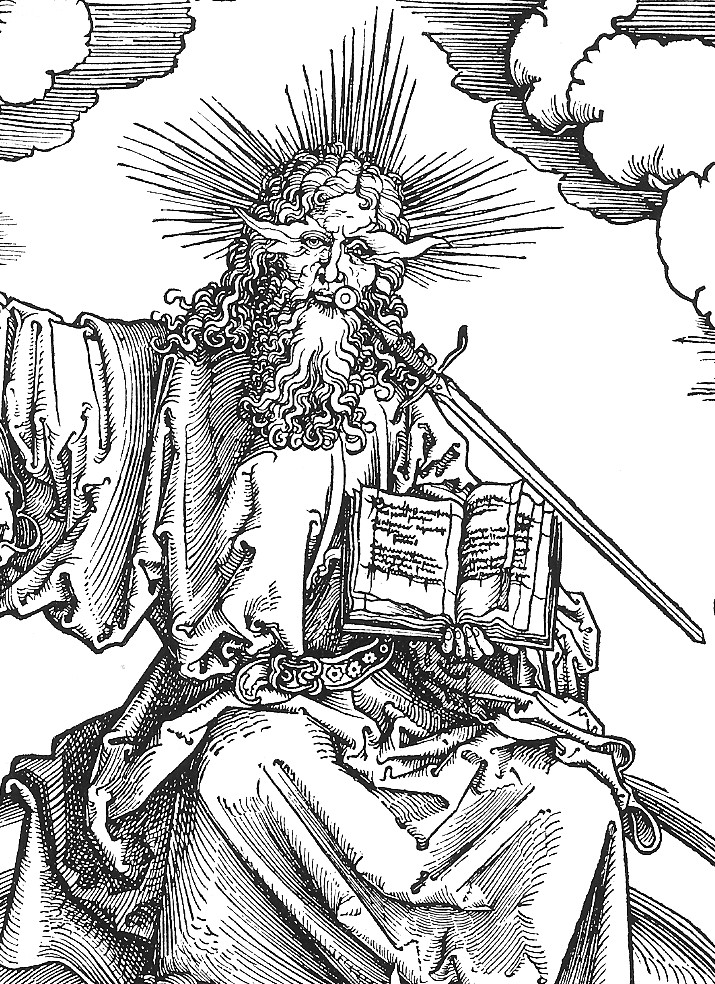
\includegraphics[width=\paperwidth,height=\paperheight]{Durer/Son_of_Man.jpg}}
   \else
     \put(0,0){\includegraphics[width=\paperwidth,height=\paperheight]{Durer/Dürer_Apocalypse_dragon.jpg}}
   \fi
}

\blankpage
\clearpage
\clearpage

\tableofcontents
\clearpage
\listoffigures
\clearpage
\ClearShipoutPicture
\chapterfigure[scale=0.35]{Durer/Durer-candlesticks.png}{St. John's Vision of the Seven Candlesticks. Albrecht Dürer, 1498.}

\pagestyle{headings}
\mainmatter
\trimFrame
\chapter{Vision of the Son of Man}
\lettrine[lines=4]{\textcolor{red}{T}}{\ he Revelation of Jesus Christ}, which God gave him to show unto his servants,%
	\cbiblefootduo{Daniel}{2:28}{there is a God in heaven that revealeth secrets, and he hath made known to the king Nebuchadnezzar what shall be in the latter days}%
			{Amos}{3:7}{Surely the Lord Jehovah will do nothing, except he reveal his secret unto his servants the prophets}%
even the things which must shortly come to pass: and he sent and signified it by his angel unto his servant John; %
\vnum{2} who bare witness of the word of God, and of the testimony of Jesus Christ, even of all things that he saw. %
\vnum{3} Blessed is he that readeth, and they that hear the words of the prophecy, and keep the things that are written therein: for the time is at hand.
\subsubsection*{Greetings to the Seven Churches}
\vnum{4} John to the seven churches that are in Asia: Grace to you and peace, from him who is%
	\cbiblefoot{Exodus}{3:14}{And God said unto Moses, I am that I am: and he said, Thus shalt thou say unto the children of Israel, I am hath sent me unto you} %
and who was and who is to come; and from the seven Spirits%
	\cbiblefoot{Isaiah}{11:2}{And the Spirit of Jehovah shall rest upon him, the spirit of wisdom and understanding, the spirit of counsel and might, the spirit of knowledge and of the fear of Jehovah}%
that are before his throne; %
\vnum{5} and from Jesus Christ, who is the faithful witness, the firstborn%
	\cbiblefoot{Psalms}{89:27}{I also will make him my first-born,
The highest of the kings of the earth} %
of the dead, and the ruler of the kings of the earth.%
	\cbiblefoot{Daniel}{7:14}{And there was given him dominion, and glory, and a kingdom, that all the peoples, nations, and languages should serve him: his dominion is an everlasting dominion, which shall not pass away, and his kingdom that which shall not be destroyed}%
Unto him that loveth us,%
	\cbiblefootduosb{Deuteronomy}{7:8}{ because Jehovah loveth you\ldots hath Jehovah brought you out with a mighty hand, and redeemed you out of the house of bondage, from the hand of Pharaoh king of Egypt}%
								{23:5}{Jehovah thy God turned the curse into a blessing unto thee, because Jehovah thy God loved thee}%
and loosed us from our sins by his blood; %
\vnum{6} and he made us to be a kingdom, to be priests%
	\cbiblefootduo{Exodus}{19:6}{ye shall be unto me a kingdom of priests, and a holy nation}%
				{Isaiah}{61:6}{ye shall be named the priests of Jehovah; men shall call you the ministers of our God: ye shall eat the wealth of the nations, and in their glory shall ye boast yourselves}%
unto his God and Father; to him be the glory and the dominion for ever and ever. Amen.%
	\cbiblefoot{Psalms}{72:18-19}{Blessed be Jehovah God, the God of Israel, who only doeth wondrous things: and blessed be his glorious name for ever; and let the whole earth be filled with his glory. Amen, and Amen}

\begin{quote}
\vnum{7} \textit{Behold, he cometh with the clouds;%
	\footnote{\cbibleref{Psalms}{18:9-12}{He bowed the heavens also, and came down; and thick darkness was under his feet. And he rode upon a cherub, and did fly; yea, he soared upon the wings of the wind. He made darkness his hiding-place, his pavilion round about him, darkness of waters, thick clouds of the skies. At the brightness before him his thick clouds passed, hailstones and coals of fire}\ldots%
				\cbibleref{Psalms}{97:1-2}{Jehovah reigneth; let the earth rejoice; let the multitude of isles be glad. Clouds and darkness are round about him}\ldots%
				\cbibleref{Isaiah}{19:1}{Behold, Jehovah rideth upon a swift cloud, and cometh unto Egypt}\ldots%
				\cbibleref{Daniel}{7:13}{there came with the clouds of heaven one like unto a son of man}\ldots%
				\cbibleref{Nahum}{1:3}{Jehovah hath his way in the whirlwind and in the storm, and the clouds are the dust of his feet}}\\%
and every eye shall see him,%
	\cbiblefootduosb{Isaiah}{52:10}{Jehovah hath made bare his holy arm in the eyes of all the nations; and all the ends of the earth have seen the salvation of our God}%
	{62:2}{And the nations shall see thy righteousness, and all kings thy glory}\\%
and they that pierced him; \\and all the tribes of the earth \\shall mourn over him.}%
	\cbiblefoot{Zechariah}{12:10-14}{they shall look unto me whom they have pierced; and they shall mourn for him, as one mourneth for his only son, and shall be in bitterness for him, as one that is in bitterness for his first-born. In that day shall there be a great mourning in Jerusalem, as the mourning of Hadadrimmon in the valley of Megiddon. And the land shall mourn, every family apart\ldots} 
\end{quote} Even so, Amen.

\vnum{8} I am the Alpha and the Omega,%
	\cbiblefootcuartosb{Isaiah}{41:4}{I, Jehovah, the first, and with the last, I am he}%
	{43:10}{I am he: before me there was no God formed, neither shall there be after me}%
	{44:6}{Thus saith Jehovah, the King of Israel, and his Redeemer, Jehovah of hosts: I am the first, and I am the last; and besides me there is no God}%
	{48:12}{I am he; I am the first, I also am the last}%
saith the Lord God, who is%
	\footnote{cf. v 4} %
and who was and who is to come, the Almighty.

\subsubsection*{Vision of Christ}

\vnum{9} I John, your brother and partaker with you in the tribulation and kingdom and patience which are in Jesus, was in the isle that is called Patmos,%
	\footnote{\cbibleref{Ezekiel}{1:1}{Now it came to pass\ldots as I was among the captives by the river Chebar, that the heavens were opened, and I saw visions of God}\ldots%
			\cbibleref{Daniel}{8:2}{And I saw in the vision; now it was so, that when I saw, I was in Shushan the palace, which is in the province of Elam; and I saw in the vision, and I was by the river Ulai}\ldots%
			\cbiblechvs{Daniel}{10:4-5}{as I was by the side of the great river, which is Hiddekel, I lifted up mine eyes, and looked, and, behold\ldots}}%
for the word of God and the testimony of Jesus. %
\vnum{10} I was in the Spirit on the Lord’s day, and I heard behind me a great voice, as of a trumpet %
\vnum{11} saying, What thou seest, write in a book%
\cbiblefoottrio{Isaiah}{30:8}{Now go, write it before them on a tablet, and inscribe it in a book, that it may be for the time to come for ever and ever}%
				{Jeremiah}{30:2}{Thus speaketh Jehovah, the God of Israel, saying, Write thee all the words that I have spoken unto thee in a book}%
				{Habakkuk}{2:2}{And Jehovah answered me, and said, Write the vision, and make it plain upon tablets, that he may run that readeth it}%
and send it to the seven churches: unto Ephesus, and unto Smyrna, and unto Pergamum, and unto Thyatira, and unto Sardis, and unto Philadelphia, and unto Laodicea.

\vnum{12} And I turned to see the voice that spake with me. And having turned I saw seven golden candlesticks;%
	\cbiblefootduo{Exodus}{25:31-40}{And thou shalt make a candlestick of pure gold\ldots And thou shalt make the lamps thereof, seven: and they shall light the lamps thereof, to give light over against it\ldots And see that thou make them after their pattern, which hath been showed thee in the mount}%
	{Zechariah}{4:2}{And he said unto me, What seest thou? And I said, I have seen, and, behold, a candlestick all of gold, with its bowl upon the top of it, and its seven lamps thereon; there are seven pipes to each of the lamps, which are upon the top thereof}
\vnum{13} and in the midst of the candlesticks one like unto a son of man,%
\cbiblefoottrio{Ezekiel}{1:26}{and upon the likeness of the throne was a likeness as the appearance of a man upon it above}%
			{Daniel}{7:13}{ I saw in the night-visions, and, behold, there came with the clouds of heaven one like unto a son of man, and he came even to the ancient of days, and they brought him near before him}%
			{Daniel}{10:16}{And, behold, one in the likeness of the sons of men touched my lips}%
clothed with a garment down to the foot, and girt about at the breasts with a golden girdle.%
	\cbiblefoot{Daniel}{10:5}{ I lifted up mine eyes, and looked, and, behold, a man clothed in linen, whose loins were girded with pure gold of Uphaz}
\vnum{14} And his head and his hair were white as white wool, white as snow;%
	\cbiblefoot{Daniel}{7:9}{I beheld till thrones were placed, and one that was ancient of days did sit: his raiment was white as snow, and the hair of his head like pure wool}%
and his eyes were as a flame of fire; %
	\cbiblefoot{Daniel}{10:6}{his face as the appearance of lightning, and his eyes as flaming torches} %
\vnum{15} and his feet like unto burnished brass, as if it had been refined in a furnace;%
	\cbiblefootduosb{Ezekiel}{1:7}{the sole of their feet\ldots sparkled like burnished brass}%
			{1:27}{And I saw as it were glowing metal, as the appearance of fire within it round about, from the appearance of his loins and upward; and from the appearance of his loins and downward I saw as it were the appearance of fire, and there was brightness round about him}%
and his voice as the voice of many waters.%
	\cbiblefootduo{Psalms}{93:3-4}{The floods have lifted up, O Jehovah, the floods have lifted up their voice; the floods lift up their waves. Above the voices of many waters, the mighty breakers of the sea, Jehovah on high is mighty}%
        		{Ezekiel}{1:24}{ I heard the noise of their wings like the noise of great waters, like the voice of the Almighty, a noise of tumult like the noise of a host}
\vnum{16} And he had in his right hand seven stars: and out of his mouth proceeded a sharp two-edged sword:%
	\cbiblefootduosb{Isaiah}{11:4}{he shall smite the earth with the rod of his mouth; and with the breath of his lips shall he slay the wicked}%
				{49:1}{he hath made my mouth like a sharp sword}
and his countenance was as the sun shineth in his strength.%
	\cbiblefootduo{Isaiah}{60:19-20}{The sun shall be no more thy light by day; neither for brightness shall the moon give light unto thee: but Jehovah will be unto thee an everlasting light, and thy God thy glory. Thy sun shall no more go down, neither shall thy moon withdraw itself; for Jehovah will be thine everlasting light, and the days of thy mourning shall be ended}%
			{Malachi}{4:2}{But unto you that fear my name shall the sun of righteousness arise with healing in its wings}

\vnum{17} And when I saw him, I fell at his feet as one dead.%
\footnote{\cbibleref{Ezekiel}{1:28}{This was the appearance of the likeness of the glory of Jehovah. And when I saw it, I fell upon my face}\ldots%
				\cbibleref{Daniel}{8:18}{Now as he was speaking with me, I fell into a deep sleep with my face toward the ground}\ldots%
				\cbiblechvs{Daniel}{10:8-9}{So I was left alone, and saw this great vision, and there remained no strength in me; for my comeliness was turned in me into corruption, and I retained no strength. Yet heard I the voice of his words; and when I heard the voice of his words, then was I fallen into a deep sleep on my face, with my face toward the ground}\ldots%
				\cbiblechvs{Daniel}{10:15-17}{And when he had spoken unto me according to these words, I set my face toward the ground, and was dumb. And, behold, one in the likeness of the sons of men touched my lips: then I opened my mouth, and spake and said unto him that stood before me, O my lord, by reason of the vision my sorrows are turned upon me, and I retain no strength. For how can the servant of this my lord talk with this my lord? for as for me, straightway there remained no strength in me, neither was there breath left in me.}}
And he laid his right hand upon me,%
	\cbiblefootduosb{Daniel}{8:18}{ I fell into a deep sleep with my face toward the ground; but he touched me, and set me upright}%
					{10:18-19}{Then there touched me again one like the appearance of a man, and he strengthened me. And he said, O man greatly beloved, fear not: peace be unto thee, be strong, yea, be strong. And when he spake unto me, I was strengthened, and said, Let my lord speak; for thou hast strengthened me}		
saying, Fear not; I am the first and the last, %
\vnum{18} and the Living one; and I was dead, and behold, I am alive for evermore, and I have the keys of death and of Hades. %
\vnum{19} Write therefore the things which thou sawest, and the things which are, and the things which shall come to pass hereafter; %
\vnum{20} the mystery of the seven stars which thou sawest in my right hand, and the seven golden candlesticks. The seven stars are the angels of the seven churches: and the seven candlesticks are seven churches.

\chapter{Letters to Ephesus, Smyrna, \newline Pergamum \& Thyatira}
\subsection*{Letter to Ephesus}
\lettrine[lines=3]{\textcolor{red}{T}}{\ o the angel of the church in Ephesus write} :

\zz These things saith he that holdeth the seven stars in his right hand, he that walketh in the midst of the seven golden candlesticks:%
	\cbiblefoot{Ezekiel}{28:14}{Thou wast the anointed cherub that covereth: and I set thee, so that thou wast upon the holy mountain of God; thou hast walked up and down in the midst of the stones of fire}
\vnum{2} I know thy works, and thy toil and patience, and that thou canst not bear evil men, and didst try them that call themselves apostles, and they are not, and didst find them false; %
\vnum{3} and thou hast patience and didst bear for my name’s sake, and hast not grown weary. %
\vnum{4} But I have this against thee, that thou didst leave thy first love.%
	\cbiblefoot{Jeremiah}{2:2-5}{Go, and cry in the ears of Jerusalem, saying, Thus saith Jehovah, I remember for thee the kindness of thy youth, the love of thine espousals; how thou wentest after me in the wilderness, in a land that was not sown. Israel was holiness unto Jehovah, the first-fruits of his increase: all that devour him shall be held guilty; evil shall come upon them, saith Jehovah\ldots Thus saith Jehovah, What unrighteousness have your fathers found in me, that they are gone far from me, and have walked after vanity, and are become vain?}
\vnum{5} Remember%
	\cbiblefoottriosb{Ezekiel}{16:61-63}{Then shalt thou remember thy ways, and be ashamed\ldots And I will establish my covenant with thee; and thou shalt know that I am Jehovah; that thou mayest remember, and be confounded, and never open thy mouth any more, because of thy shame, when I have forgiven thee all that thou hast done, saith the Lord Jehovah}%
				{20:43}{And there shall ye remember your ways, and all your doings, wherein ye have polluted yourselves; and ye shall loathe yourselves in your own sight for all your evils that ye have committed}%
				{36:31}{Then shall ye remember your evil ways, and your doings that were not good; and ye shall loathe yourselves in your own sight for your iniquities and for your abominations}%
therefore whence thou art fallen, and repent and do the first works; or else I come to thee, and will move thy candlestick out of its place, except thou repent. %
\vnum{6} But this thou hast, that thou hatest the works of the Nicolaitans, which I also hate.%
	\cbiblefoottriosb{Psalms}{26:5}{I hate the assembly of evil-doers, and will not sit with the wicked}%
			{101:3}{I hate the work of them that turn aside; it shall not cleave unto me}%
			{139:21}{Do not I hate them, O Jehovah, that hate thee? And am not I grieved with those that rise up against thee?} %
\vnum{7} He that hath an ear, let him hear what the Spirit saith to the churches. To him that overcometh, to him will I give to eat of the tree of life, which is in the Paradise of God.%
	\cbiblefootduosb{Genesis}{2:9}{And out of the ground made Jehovah God to grow every tree that is pleasant to the sight, and good for food; the tree of life also in the midst of the garden}%
				{3:22-24}{And Jehovah God said, Behold, the man is become as one of us, to know good and evil; and now, lest he put forth his hand, and take also of the tree of life, and eat, and live for ever— therefore Jehovah God sent him forth from the garden of Eden, to till the ground from whence he was taken. So he drove out the man; and he placed at the east of the garden of Eden the Cherubim, and the flame of a sword which turned every way, to keep the way of the tree of life}
\subsection*{Letter to Smyrna}
\vnum{8} And to the angel of the church in Smyrna write:

These things saith the first and the last, who was dead, and lived again: %
\vnum{9} I know thy tribulation, and thy poverty (but thou art rich), and the blasphemy of them that say they are Jews, and they are not, but are a synagogue of Satan. %
\vnum{10} Fear not the things which thou art about to suffer: behold, the devil is about to cast some of you into prison, that ye may be tried; and ye shall have tribulation ten days.%
	\cbiblefoot{Daniel}{1:12, 14}{Prove thy servants, I beseech thee, ten days; and let them give us pulse to eat, and water to drink\ldots So he hearkened unto them in this matter, and proved them ten days.}%
 Be thou faithful unto death, and I will give thee the crown of life. %
\vnum{11} He that hath an ear, let him hear what the Spirit saith to the churches. He that overcometh shall not be hurt of the second death.
\subsection*{Letter to Pergamum}
\vnum{12} And to the angel of the church in Pergamum write:

These things saith he that hath the sharp two-edged sword:%
	\cbiblefoot{Isaiah}{49:2}{He hath made my mouth like a sharp sword}%
\vnum{13} I know where thou dwellest,%
	\cbiblefoot{Ezekiel}{12:2}{Thou dwellest in the midst of the rebellious house, that have eyes to see, and see not, that have ears to hear, and hear not; for they are a rebellious house.}
 even where Satan’s throne is; and thou holdest fast my name, and didst not deny my faith, even in the days of Antipas my witness, my faithful one, who was killed among you, where Satan dwelleth. %
\vnum{14} But I have a few things against thee, because thou hast there some that hold the teaching of Balaam, who taught Balak to cast a stumblingblock before the children of Israel, to eat things sacrificed to idols, and to commit fornication.%
		\cbiblefootduosb{Numbers}{31:15-16}{Moses said unto them, Have ye saved all the women alive? Behold, these caused the children of Israel, through the counsel of Balaam, to commit trespass against Jehovah in the matter of Peor}%
								{25:1-2}{The people began to play the harlot with the daughters of Moab: for they called the people unto the sacrifices of their gods; and the people did eat, and bowed down to their gods.}
\vnum{15} So hast thou also some that hold the teaching of the Nicolaitans in like manner. %
\vnum{16} Repent therefore; or else I come to thee quickly, and I will make war against them with the sword of my mouth.%
	\cbiblefoot{Jeremiah}{21:5}{I myself will fight against you with an outstretched hand and with a strong arm, even in anger, and in wrath, and in great indignation}
\vnum{17} He that hath an ear, let him hear what the Spirit saith to the churches. To him that overcometh, to him will I give of the hidden manna,%
	\cbiblefoot{Exodus}{16:32-34}{Moses said, This is the thing which Jehovah hath commanded, Let an omerful of it be kept throughout your generations, that they may see the bread wherewith I fed you in the wilderness, when I brought you forth from the land of Egypt. And Moses said unto Aaron, Take a pot, and put an omerful of manna therein, and lay it up before Jehovah, to be kept throughout your generations. As Jehovah commanded Moses, so Aaron laid it up before the Testimony, to be kept} 
and I will give him a white stone, and upon the stone a new name written, which no one knoweth but he that receiveth it.
	\cbiblefoottriosb{Isaiah}{56:4-5}{Thus saith Jehovah of the eunuchs that keep my sabbaths, and choose the things that please me, and hold fast my covenant: Unto them will I give in my house and within my walls a memorial and a name better than of sons and of daughters; I will give them an everlasting name, that shall not be cut off.}%
					{62:2}{The nations shall see thy righteousness, and all kings thy glory, and thou shalt be called by a new name, which the mouth of Jehovah shall name}
					{65:15}{Ye shall leave your name for a curse unto my chosen; and the Lord Jehovah will slay thee; and he will call his servants by another name}
\subsection*{Letter to Thyatira}
\vnum{18} And to the angel of the church in Thyatira write:

These things saith the Son of God, who hath his eyes like a flame of fire, and his feet are like unto burnished brass:\footnote{cf. 1:14-15} %
\vnum{19} I know thy works, and thy love and faith and ministry and patience, and that thy last works are more than the first. %
\vnum{20} But I have this against thee, that thou sufferest the woman Jezebel, who calleth herself a prophetess; and she teacheth and seduceth my servants to commit fornication, and to eat things sacrificed to idols.%
	\cbiblefootduo{IKings}{16:31}{As if it had been a light thing for him to walk in the sins of Jeroboam\ldots, he took to wife Jezebel the daughter of Ethbaal king of the Sidonians, and went and served Baal, and worshipped him}%
				 {IIKings}{9:22}{When Joram saw Jehu\ldots he said, Is it peace, Jehu? And he answered, What peace, so long as the whoredoms of thy mother Jezebel and her witchcrafts are so many?}
\vnum{21} And I gave her time that she should repent; and she willeth not to repent of her fornication. %
\vnum{22} Behold, I cast her into a bed, and them that commit adultery with her into great tribulation, except they repent of her works. %
\vnum{23} And I will kill her children with death; and all the churches shall know that I am he that searcheth the reins and hearts:%
	\cbiblefoot{Jeremiah}{11:20}{O Jehovah of hosts, who judgest righteously, who triest the heart and the mind, I shall see thy vengeance on them}
 and I will give unto each one of you according to your works. %
\vnum{24} But to you I say, to the rest that are in Thyatira, as many as have not this teaching, who know not the deep things of Satan, as they are wont to say; I cast upon you none other burden. %
\vnum{25} Nevertheless that which ye have, hold fast till I come. %
\vnum{26} And he that overcometh, and he that keepeth my works unto the end, to him will I give authority over the nations: %
\vnum{27} and he shall rule them with a rod of iron, as the vessels of the potter are broken to shivers;%
	\cbiblefoot{Psalms}{2:8-9}{Ask of me, and I will give thee the nations for thine inheritance, And the uttermost parts of the earth for thy possession. Thou shalt break them with a rod of iron; Thou shalt dash them in pieces like a potter’s vessel.}
 as I also have received of my Father: %
\vnum{28} and I will give him the morning star. %
\vnum{29} He that hath an ear, let him hear what the Spirit saith to the churches.

\chapter{Letters to Sardis, Philadelphia \& Laodicea}
\subsection*{Letter to Sardis}
\lettrine[lines=3]{\textcolor{red}{A}}{\ nd to the angel of the church in Sardis write}:

\zz These things saith he that hath the seven Spirits of God, and the seven stars: I know thy works, that thou hast a name that thou livest, and thou art dead. %
\vnum{2} Be thou watchful, and establish the things that remain, which were ready to die: for I have found no works of thine perfected before my God. %
\vnum{3} Remember therefore how thou hast received and didst hear; and keep it, and repent. If therefore thou shalt not watch, I will come as a thief, and thou shalt not know what hour I will come upon thee. %
\vnum{4} But thou hast a few names in Sardis that did not defile their garments: and they shall walk with me in white; for they are worthy. %
\vnum{5} He that overcometh shall thus be arrayed in white garments; and I will in no wise blot his name out of the book of life,%
	\footnote{\cbibleref{Exodus}{32:32-33}{Yet now, if thou wilt forgive their sin—; and if not, blot me, I pray thee, out of thy book which thou hast written. And Jehovah said unto Moses, Whosoever hath sinned against me, him will I blot out of my book.}\ldots%
			\cbibleref{Psalms}{69:28}{Let them be blotted out of the book of life, And not be written with the righteous.}\ldots%
			\cbibleref{Daniel}{12:1}{Thy people shall be delivered, every one that shall be found written in the book.}\ldots%
			\cbibleref{Malachi}{3:16}{Then they that feared Jehovah spake one with another; and Jehovah hearkened, and heard, and a book of remembrance was written before him, for them that feared Jehovah, and that thought upon his name.}}
 and I will confess his name before my Father, and before his angels. %
\vnum{6} He that hath an ear, let him hear what the Spirit saith to the churches.
\subsection*{Letter to Philadelphia}
\vnum{7} And to the angel of the church in Philadelphia write:

These things saith he that is holy, he that is true, he that hath the key of David, he that openeth and none shall shut, and that shutteth and none openeth:%
	\cbiblefootduo{Isaiah}{22:20-23}{It shall come to pass in that day, that I will call my servant Eliakim\ldots and I will commit thy government into his hand; and he shall be a father to the inhabitants of Jerusalem, and to the house of Judah. And the key of the house of David will I lay upon his shoulder; and he shall open, and none shall shut; and he shall shut, and none shall open. And I will fasten him as a nail in a sure place; and he shall be for a throne of glory to his father’s house.}%
				{Job}{12:14}{With God is wisdom and might\ldots Behold, he breaketh down, and it cannot be built again; He shutteth up a man, and there can be no opening.}
\vnum{8} I know thy works (behold, I have set before thee a door opened, which none can shut), that thou hast a little power, and didst keep my word, and didst not deny my name.  \vnum{9} Behold, I give of the synagogue of Satan, of them that say they are Jews, and they are not, but do lie; behold, I will make them to come and worship before thy feet,%
	\footnote{\cbibleref{Isaiah}{49:23}{Kings shall be thy nursing fathers, and their queens thy nursing mothers: they shall bow down to thee with their faces to the earth, and lick the dust of thy feet; and thou shalt know that I am Jehovah; and they that wait for me shall not be put to shame}\ldots%
				\cbiblechvs{Isaiah}{60:14}{The sons of them that afflicted thee shall come bending unto thee; and all they that despised thee shall bow themselves down at the soles of thy feet; and they shall call thee The city of Jehovah, The Zion of the Holy One of Israel.}}
 and to know that I have loved thee. %
 	\cbiblefoot{Isaiah}{43:4}{Since thou hast been precious in my sight, and honorable, and I have loved thee; therefore will I give men in thy stead, and peoples instead of thy life.}
\vnum{10} Because thou didst keep the word of my patience, I also will keep thee from the hour of trial, that hour which is to come upon the whole world, to try them that dwell upon the earth. %
\vnum{11} I come quickly: hold fast that which thou hast, that no one take thy crown. %
\vnum{12} He that overcometh, I will make him a pillar in the temple of my God, and he shall go out thence no more: and I will write upon him the name of my God, and the name of the city of my God,%
	\cbiblefoot{Ezekiel}{48:35}{The name of the city from that day shall be, Jehovah is there.}
 the new Jerusalem, which cometh down out of heaven from my God, and mine own new name. %
\vnum{13} He that hath an ear, let him hear what the Spirit saith to the churches.
\subsection*{Letter to Laodicea}
\vnum{14} And to the angel of the church in Laodicea write:

These things saith the Amen, the faithful and true witness,%
	\cbiblefoot{Isaiah}{65:16}{He who blesseth himself in the earth shall bless himself in the God of truth; and he that sweareth in the earth shall swear by the God of truth}
 the beginning of the creation of God:%
 	\cbiblefoot{Proverbs}{8:22-23}{Jehovah possessed me in the beginning of his way, before his works of old. I was set up from everlasting, from the beginning, before the earth was.} %
\vnum{15} I know thy works, that thou art neither cold nor hot: I would thou wert cold or hot. %
\vnum{16} So because thou art lukewarm, and neither hot nor cold, I will spew thee out of my mouth. %
\vnum{17} Because thou sayest, I am rich,%
	\cbiblefootduo{Zechariah}{11:4-5}{Thus said Jehovah my God: Feed the flock of slaughter; whose possessors slay them, and hold themselves not guilty; and they that sell them say, Blessed be Jehovah, for I am rich; and their own shepherds pity them not.}	
				{Hosea}{12:8-9}{Ephraim said, Surely I am become rich, I have found me wealth: in all my labors they shall find in me no iniquity that were sin. But I am Jehovah thy God from the land of Egypt; I will yet again make thee to dwell in tents, as in the days of the solemn feast.}
 and have gotten riches, and have need of nothing; and knowest not that thou art the wretched one and miserable and poor and blind and naked: %
\vnum{18} I counsel thee to buy of me gold refined by fire, that thou mayest become rich; and white garments, that thou mayest clothe thyself, and that the shame of thy nakedness be not made manifest; and eyesalve to anoint thine eyes, that thou mayest see.%
	\cbiblefoot{Isaiah}{55:1-3}{Ho, every one that thirsteth, come ye to the waters, and he that hath no money; come ye, buy, and eat; yea, come, buy wine and milk without money and without price. Wherefore do ye spend money for that which is not bread? and your labor for that which satisfieth not? hearken diligently unto me, and eat ye that which is good, and let your soul delight itself in fatness. Incline your ear, and come unto me; hear, and your soul shall live: and I will make an everlasting covenant with you, even the sure mercies of David} %
\vnum{19} As many as I love, I reprove and chasten:%
	\cbiblefoot{Proverbs}{3:11-12}{My son, despise not the chastening of Jehovah; neither be weary of his reproof: for whom Jehovah loveth he reproveth, even as a father the son in whom he delighteth.}
 be zealous therefore, and repent. %
\vnum{20} Behold, I stand at the door and knock:%
	\cbiblefoot{SongofSongs}{5:2}{I was asleep, but my heart waked: it is the voice of my beloved that knocketh, saying, open to me, my sister, my love, my dove, my undefiled; for my head is filled with dew, my locks with the drops of the night.}
 if any man hear my voice and open the door, I will come in to him, and will sup with him, and he with me. %
\vnum{21} He that overcometh, I will give to him to sit down with me in my throne, as I also overcame, and sat down with my Father in his throne. %
\vnum{22} He that hath an ear, let him hear what the Spirit saith to the churches.

\chapterfigure[scale=0.25]{Durer/Dürer_-_Saint_John_before_God_and_the_Elders.jpg}{St. John before God and the Elders. Dürer, 1498.}

\chapter{Vision of God's Throne}
\lettrine[lines=3,slope=0.5em]{\textcolor{red}{A}}{\ fter these things I saw}, and behold, a door opened in heaven, and the first voice that I heard, a voice as of a trumpet speaking with me, one saying, Come up hither, and I will show thee the things which must come to pass hereafter.%
	\footnote{cf. 1:1} %
\vnum{2} Straightway I was in the Spirit: and behold, there was a throne set in heaven, and one sitting upon the throne;%
	\footnote{\cbibleref{IKings}{22:19}{I saw Jehovah sitting on his throne, and all the host of heaven standing by him on his right hand and on his left}\ldots%
			(cf. \textbf{\ibibleverse[textit]{IIChronicles}(18:18)})\ldots
			\cbibleref{Psalms}{11:4}{Jehovah is in his holy temple; Jehovah, his throne is in heaven}\ldots%
			\cbiblechvs{Psalms}{47:8}{God reigneth over the nations: God sitteth upon his holy throne.}\ldots%
			\cbiblechvs{Psalms}{103:19}{Jehovah hath established his throne in the heavens; and his kingdom ruleth over all.}\ldots%
			\cbibleref{Ezekiel}{1:26}{Above the firmament that was over their heads was the likeness of a throne, as the appearance of a sapphire stone; and upon the likeness of the throne was a likeness as the appearance of a man upon it above.}\ldots%
			\cbiblechvs{Ezekiel}{10:1}{Then I looked, and, behold, in the firmament that was over the head of the cherubim there appeared above them as it were a sapphire stone, as the appearance of the likeness of a throne.}\ldots%
			\cbibleref{Isaiah}{6:1}{I saw the Lord sitting upon a throne, high and lifted up}} %
\vnum{3} and he that sat was to look upon like a jasper stone and a sardius: and there was a rainbow round about the throne,%
	\cbiblefoot{Ezekiel}{1:28}{As the appearance of the bow that is in the cloud in the day of rain, so was the appearance of the brightness round about. This was the appearance of the likeness of the glory of Jehovah.}
 like an emerald to look upon. %
\vnum{4} And round about the throne were four and twenty thrones: and upon the thrones I saw four and twenty elders sitting,%
	\cbiblefoot{Isaiah}{24:23}{Then the moon shall be confounded, and the sun ashamed; for Jehovah of hosts will reign in mount Zion, and in Jerusalem; and before his elders shall be glory.}
 arrayed in white garments; and on their heads crowns of gold. %
\vnum{5} And out of the throne proceed lightnings and voices and thunders.%
	\cbiblefoot{Exodus}{19:16-17}{There were thunders and lightnings, and a thick cloud upon the mount, and the voice of a trumpet exceeding loud; and all the people that were in the camp trembled. 17 And Moses brought forth the people out of the camp to meet God}
 And there were seven lamps of fire burning before the throne,%
 	\cbiblefootduo{Ezekiel}{1:13}{As for the likeness of the living creatures, their appearance was like burning coals of fire, like the appearance of torches: the fire went up and down among the living creatures; and the fire was bright, and out of the fire went forth lightning}
 				{Zechariah}{4:2}{Behold, a candlestick all of gold, with its bowl upon the top of it, and its seven lamps thereon}
  which are the seven Spirits of God; %
\vnum{6} and before the throne, as it were a sea of glass like unto crystal;%
	\cbiblefoot{Ezekiel}{1:22}{And over the head of the living creature there was the likeness of a firmament, like the terrible crystal to look upon, stretched forth over their heads above.}
 and in the midst of the throne, and round about the throne, four living creatures%
 	\cbiblefoot{Ezekiel}{1:5}{And out of the midst thereof came the likeness of four living creatures}
  full of eyes before and behind.%
  	\cbiblefoot{Ezekiel}{10:12}{And their whole body, and their backs, and their hands, and their wings, and the wheels, were full of eyes round about, even the wheels that they four had.}
\vnum{7} And the first creature was like a lion, and the second creature like a calf, and the third creature had a face as of a man, and the fourth creature was like a flying eagle.%
	\cbiblefootduosb{Ezekiel}{1:10}{As for the likeness of their faces, they had the face of a man; and they four had the face of a lion on the right side; and they four had the face of an ox on the left side; they four had also the face of an eagle.}%
					{10:14}{Every one had four faces: the first face was the face of the cherub, and the second face was the face of a man, and the third the face of a lion, and the fourth the face of an eagle.} %
\vnum{8} And the four living creatures, having each one of them six wings, are full of eyes round about and within: and they have no rest day and night, saying,

Holy, holy, holy, is the Lord God, the Almighty, who was and who is and who is to come.%
	\cbiblefoot{Isaiah}{6:2-3}{Above him stood the seraphim: each one had six wings; with twain he covered his face, and with twain he covered his feet, and with twain he did fly. And one cried unto another, and said, Holy, holy, holy, is Jehovah of hosts: the whole earth is full of his glory. And the foundations of the thresholds shook at the voice of him that cried, and the house was filled with smoke.} 

\vnum{9} And when the living creatures shall give glory and honor and thanks to him that sitteth on the throne, to him that liveth for ever and ever,%
	\cbiblefoot{Daniel}{12:7}{He held up his right hand and his left hand unto heaven, and sware by him that liveth for ever} %
\vnum{10} the four and twenty elders shall fall down before him that sitteth on the throne, and shall worship him that liveth for ever and ever, and shall cast their crowns before the throne, saying,

\vnum{11} Worthy art thou, our Lord and our God, to receive the glory and the honor and the power: for thou didst create all things, and because of thy will they were, and were created.%
	\cbiblefoot{IChronicles}{29:11-13}{Thine, O Jehovah, is the greatness, and the power, and the glory, and the victory, and the majesty: for all that is in the heavens and in the earth is thine; thine is the kingdom, O Jehovah, and thou art exalted as head above all. Both riches and honor come of thee, and thou rulest over all; and in thy hand is power and might; and in thy hand it is to make great, and to give strength unto all. Now therefore, our God, we thank thee, and praise thy glorious name.}


\chapter{Worthy is the Lamb}
\lettrine[lines=3,slope=0.5em]{\textcolor{red}{A}}{\ nd I saw} in the right hand of him that sat on the throne a book written within and on the back, close sealed with seven seals.%
 \cbiblefoottrio{Ezekiel}{2:9-10}{A scroll of a book was therein; and he spread it before me: and it was written within and without; and there were written therein lamentations, and mourning, and woe}%
 					{Isaiah}{29:11-12}{All vision is become unto you as the words of a book that is sealed, which men deliver to one that is learned, saying, Read this, I pray thee; and he saith, I cannot, for it is sealed: and the book is delivered to him that is not learned, saying, Read this, I pray thee; and he saith, I am not learned}%
 					{Daniel}{12:4, 9}{But thou, O Daniel, shut up the words, and seal the book, even to the time of the end\ldots Go thy way, Daniel; for the words are shut up and sealed till the time of the end.} %
\vnum{2} And I saw a strong angel proclaiming with a great voice, Who is worthy to open the book, and to loose the seals thereof? %
\vnum{3} And no one in the heaven, or on the earth, or under the earth, was able to open the book, or to look thereon. %
\vnum{4} And I wept much, because no one was found worthy to open the book, or to look thereon: %
\vnum{5} and one of the elders saith unto me, Weep not; behold, the Lion that is of the tribe of Judah,%
	\cbiblefoot{Genesis}{49:9}{Judah is a lion's whelp; from the prey, my son, thou art gone up: He stooped down, he couched as a lion, and as a lioness; who shall rouse him up?}
 the Root of David%
 	\cbiblefoot{Isaiah}{11:1, 10}{And there shall come forth a shoot out of the stock of Jesse, and a branch out of his roots shall bear fruit\ldots And it shall come to pass in that day, that the root of Jesse, that standeth for an ensign of the peoples, unto him shall the nations seek; and his resting-place shall be glorious.}
 , hath overcome to open the book and the seven seals thereof. %
\vnum{6} And I saw in the midst of the throne and of the four living creatures, and in the midst of the elders, a Lamb standing, as though it had been slain,%
	\cbiblefootduo{Isaiah}{53:7}{As a lamb that is led to the slaughter, and as a sheep that before its shearers is dumb, so he opened not his mouth}%
					  {Jeremiah}{11:19}{I was like a gentle lamb that is led to the slaughter}
 having seven horns, and seven eyes, which are the seven Spirits of God, sent forth into all the earth.%
 	\cbiblefoot{Zechariah}{4:10}{These seven shall rejoice\ldots these are the eyes of Jehovah, which run to and fro through the whole earth.} %
\vnum{7} And he came, and he taketh it out of the right hand of him that sat on the throne. %
\vnum{8} And when he had taken the book, the four living creatures and the four and twenty elders fell down before the Lamb, having each one a harp, and golden bowls full of incense, which are the prayers of the saints.%
	\cbiblefoot{Psalms}{141:2}{Let my prayer be set forth as incense before thee; the lifting up of my hands as the evening sacrifice.} %
\vnum{9} And they sing a new song,%
	\footnote{\cbibleref{Psalms}{33:3}{Sing unto him a new song; Play skilfully with a loud noise}\ldots%
			\cbiblechvs{Psalms}{40:3}{And he hath put a new song in my mouth, even praise unto our God: many shall see it, and fear, And shall trust in Jehovah}\ldots%
			\cbiblechvs{Psalms}{96:1}{Oh sing unto Jehovah a new song: sing unto Jehovah, all the earth}\ldots%
			\cbiblechvs{Psalms}{98:1}{Oh sing unto Jehovah a new song; for he hath done marvellous things: His right hand, and his holy arm, hath wrought salvation for him}\ldots%
			\cbiblechvs{Psalms}{144:9}{I will sing a new song unto thee, O God: upon a psaltery of ten strings will I sing praises unto thee.}\ldots%
			\cbiblechvs{Psalms}{149:1}{Praise ye Jehovah. Sing unto Jehovah a new song, and his praise in the assembly of the saints}\ldots%
			\cbibleref{Isaiah}{42:10}{Sing unto Jehovah a new song, and his praise from the end of the earth; ye that go down to the sea, and all that is therein, the isles, and the inhabitants thereof.}
	}
 saying,

Worthy art thou to take the book, and to open the seals thereof: for thou wast slain, and didst purchase unto God with thy blood men of every tribe, and tongue, and people, and nation, %
\vnum{10} and madest them to be unto our God a kingdom and priests;%
	\cbiblefootduo{Exodus}{19:5-6}{Ye shall be mine own possession from among all peoples\ldots and ye shall be unto me a kingdom of priests, and a holy nation.}%
				{Isaiah}{61:6-7}{Ye shall be named the priests of Jehovah; men shall call you the ministers of our God: ye shall eat the wealth of the nations, and in their glory shall ye boast yourselves. Instead of your shame ye shall have double; and instead of dishonor they shall rejoice in their portion: therefore in their land they shall possess double; everlasting joy shall be unto them.}
 and they reign upon the earth.

\vnum{11} And I saw, and I heard a voice of many angels round about the throne and the living creatures and the elders; and the number of them was ten thousand times ten thousand, and thousands of thousands;%
	\cbiblefoot{Daniel}{7:9-10}{I beheld till thrones were placed, and one that was ancient of days did sit\ldots Thousands of thousands ministered unto him, and ten thousand times ten thousand stood before him: the judgment was set, and the books were opened.}
\vnum{12} saying with a great voice,

Worthy is the Lamb that hath been slain to receive the power, and riches, and wisdom, and might, and honor, and glory, and blessing.

\vnum{13} And every created thing which is in the heaven, and on the earth, and under the earth, and on the sea, and all things that are in them, heard I saying,

Unto him that sitteth on the throne, and unto the Lamb, be the blessing, and the honor, and the glory, and the dominion, for ever and ever.

\vnum{14} And the four living creatures said, Amen. And the elders fell down and worshipped.

\chapterfigureB[scale=0.2]{Durer/Durer_Revelation_Four_Riders.jpg}{The Four Horsemen. Albrecht Dürer, 1498.}

\chapter{The First Six Seals}
\subsubsection*{The First Seal}
\lettrine[lines=3]{\textcolor{red}{A}}{\ nd I saw} when the Lamb opened one of the seven seals, and I heard one of the four living creatures saying as with a voice of thunder, Come. 
\vnum{2} And I saw, and behold, a white horse,%
	\cbiblefootduosb{Zechariah}{1:8-11}{I saw in the night, and, behold, a man riding upon a red horse, and he stood among the myrtle-trees\ldots and behind him there were horses, red, sorrel, and white\ldots And the man that stood among the myrtle-trees\ldots said, These are they whom Jehovah hath sent to walk to and fro through the earth. And they answered the angel of Jehovah\ldots We have walked to and fro through the earth, and, behold, all the earth sitteth still, and is at rest}%
					{6:1-8}{There came four chariots out from between two mountains\ldots In the first chariot were red horses; and in the second chariot black horses; and in the third chariot white horses; and in the fourth chariot grizzled strong horses\ldots These are the four winds of heaven, which go forth from standing before the Lord of all the earth\ldots and he said, Get you hence, walk to and fro through the earth}
 and he that sat thereon had a bow; and there was given unto him a crown: and he came forth conquering, and to conquer.
\subsubsection*{The Second Seal}
\vnum{3} And when he opened the second seal, I heard the second living creature saying, Come. %
\vnum{4} And another horse came forth, a red horse: and to him that sat thereon it was given to take peace from the earth, and that they should slay one another: and there was given unto him a great sword.
\subsubsection*{The Third Seal}
\vnum{5} And when he opened the third seal, I heard the third living creature saying, Come. And I saw, and behold, a black horse; and he that sat thereon had a balance in his hand. \vnum{6} And I heard as it were a voice in the midst of the four living creatures saying, A measure of wheat for a shilling, and three measures of barley for a shilling; and the oil and the wine hurt thou not.
\subsubsection*{The Fourth Seal}
\vnum{7} And when he opened the fourth seal, I heard the voice of the fourth living creature saying, Come. %
\vnum{8} And I saw, and behold, a pale horse: and he that sat upon him, his name was Death; and Hades followed with him. And there was given unto them authority over the fourth part of the earth, to kill with sword, and with famine, and with death, and by the wild beasts of the earth.
	\footnote{\cbibleref{Ezekiel}{5:12, 17}{A third part of thee shall die with the pestilence, and with famine shall they be consumed in the midst of thee; and a third part shall fall by the sword round about thee; and a third part I will scatter unto all the winds, and will draw out a sword after them\ldots I will send upon you famine and evil beasts, and they shall bereave thee; and pestilence and blood shall pass through thee; and I will bring the sword upon thee: I, Jehovah, have spoken it}\ldots%
			\cbiblechvs{Ezekiel}{14:21}{How much more when I send my four sore judgments upon Jerusalem, the sword, and the famine, and the evil beasts, and the pestilence, to cut off from it man and beast!}\ldots%
			\cbiblechvs{Ezekiel}{33:27}{Thus saith the Lord Jehovah: As I live, surely they that are in the waste places shall fall by the sword; and him that is in the open field will I give to the beasts to be devoured; and they that are in the strongholds and in the caves shall die of the pestilence.}\ldots%
			\cbibleref{Jeremiah}{14:12}{ I will consume them by the sword, and by the famine, and by the pestilence}\ldots%
			\cbiblechvs{Jeremiah}{15:2-3}{Thus saith Jehovah: Such as are for death, to death; and such as are for the sword, to the sword; and such as are for the famine, to the famine; and such as are for captivity, to captivity. And I will appoint over them four kinds, saith Jehovah: the sword to slay, and the dogs to tear, and the birds of the heavens, and the beasts of the earth, to devour and to destroy.}
			}%
\subsubsection*{The Fifth Seal}
\vnum{9} And when he opened the fifth seal, I saw underneath the altar the souls of them that had been slain for the word of God, and for the testimony which they held: %
\vnum{10} and they cried with a great voice, saying, How long, O Master, the holy and true,%
	\cbiblefootduo{Psalms}{79:1-6}{O God, the nations are come into thine inheritance; thy holy temple have they defiled\ldots The dead bodies of thy servants have they given to be food unto the birds of the heavens, the flesh of thy saints unto the beasts of the earth. Their blood have they shed like water\ldots And there was none to bury them\ldots How long, O Jehovah? wilt thou be angry for ever? Shall thy jealousy burn like fire? Pour out thy wrath upon the nations that know thee not, and upon the kingdoms that call not upon thy name.}%
				{Zechariah}{1:12}{O Jehovah of hosts, how long wilt thou not have mercy on Jerusalem and on the cities of Judah, against which thou hast had indignation these threescore and ten years?}
 dost thou not judge and avenge our blood on them that dwell on the earth?%
 	\footnote{\cbibleref{Psalms}{79:10-13}{Wherefore should the nations say, Where is their God? Let the avenging of the blood of thy servants which is shed be known among the nations in our sight\ldots Preserve thou those that are appointed to death; and render unto our neighbors sevenfold into their bosom their reproach, wherewith they have reproached thee, O Lord. So we thy people and sheep of thy pasture will give thee thanks for ever: we will show forth thy praise to all generations.}
 	} %
\vnum{11} And there was given them to each one a white robe; and it was said unto them, that they should rest yet for a little time, until their fellow-servants also and their brethren, who should be killed even as they were, should have fulfilled their course.
\subsubsection*{The Sixth Seal}
\vnum{12} And I saw when he opened the sixth seal, and there was a great earthquake;%
	\cbibleref{Ezekiel}{38:19-20}{In my jealousy and in the fire of my wrath have I spoken, surely in that day there shall be a great shaking in the land of Israel; so that the fishes of the sea, and the birds of the heavens, and the beasts of the field, and all creeping things that creep upon the earth, and all the men that are upon the face of the earth, shall shake at my presence, and the mountains shall be thrown down, and the steep places shall fall, and every wall shall fall to the ground.}
 and the sun became black as sackcloth of hair, and the whole moon became as blood;
 	\footnote{
 		\cbibleref{Joel}{3:14-16}{The day of Jehovah is near in the valley of decision. The sun and the moon are darkened, and the stars withdraw their shining. And Jehovah will roar from Zion\ldots and the heavens and the earth shall shake}\ldots%
 		\cbibleref{Isaiah}{13:9-11, 13}{Behold, the day of Jehovah cometh, cruel, with wrath and fierce anger; to make the land a desolation, and to destroy the sinners thereof out of it. For the stars of heaven and the constellations thereof shall not give their light; the sun shall be darkened in its going forth, and the moon shall not cause its light to shine. And I will punish the world for their evil\ldots I will make the heavens to tremble, and the earth shall be shaken out of its place, in the wrath of Jehovah of hosts, and in the day of his fierce anger.}\ldots%
 		\cbiblechvs{Isaiah}{50:2-3}{Behold, at my rebuke\ldots I clothe the heavens with blackness, and I make sackcloth their covering.}\ldots% 		
 		\cbibleref{Ezekiel}{32:7-9}{When I shall extinguish thee, I will cover the heavens, and make the stars thereof dark; I will cover the sun with a cloud, and the moon shall not give its light. All the bright lights of heaven will I make dark over thee, and set darkness upon thy land, saith the Lord Jehovah. I will also vex the hearts of many peoples, when I shall bring thy destruction among the nations}%
 	} %
\vnum{13} and the stars of the heaven fell unto the earth, as a fig tree casteth her unripe figs when she is shaken of a great wind.
	\cbiblefoot{Isaiah}{34:2-6}{Jehovah hath indignation against all the nations, and wrath against all their host: he hath utterly destroyed them, he hath delivered them to the slaughter\ldots And all the host of heaven shall be dissolved, and the heavens shall be rolled together as a scroll; and all their host shall fade away, as the leaf fadeth from off the vine, and as a fading leaf from the fig-tree. For my sword hath drunk its fill in heaven: behold, it shall come down upon\ldots the people of my curse, to judgment.} %
\vnum{14} And the heaven was removed as a scroll when it is rolled up; and every mountain and island were moved out of their places.
	\cbiblefoot{Ezekiel}{26:15}{Thus saith the Lord Jehovah to Tyre: shall not the isles shake at the sound of thy fall, when the wounded groan, when the slaughter is made in the midst of thee?} %
\vnum{15} And the kings of the earth, and the princes, and the chief captains, and the rich, and the strong,%
	\cbiblefootduosb{Isaiah}{24:21}{Jehovah will punish the host of the high ones on high, and the kings of the earth upon the earth}%
					{34:12}{They shall call the nobles thereof to the kingdom, but none shall be there; and all its princes shall be nothing}
 and every bondman and freeman, hid themselves in the caves and in the rocks of the mountains;%
 	\footnote{\cbibleref{Isaiah}{2:9-12}{The mean man is bowed down, and the great man is brought low: therefore forgive them not. Enter into the rock, and hide thee in the dust, from before the terror of Jehovah, and from the glory of his majesty. For there shall be a day of Jehovah of hosts upon all that is proud and haughty, and upon all that is lifted up; and it shall be brought low}\ldots%
 			\cbiblevs{Isaiah}{2:19-21}{And men shall go into the caves of the rocks, and into the holes of the earth, from before the terror of Jehovah, and from the glory of his majesty, when he ariseth to shake mightily the earth. In that day men shall cast away their idols\ldots to go into the caverns of the rocks, and into the clefts of the ragged rocks, from before the terror of Jehovah, and from the glory of his majesty, when he ariseth to shake mightily the earth.}		
 	}
\vnum{16} and they say to the mountains and to the rocks, Fall on us, and hide us from the face of him that sitteth on the throne, and from the wrath of the Lamb: %
\vnum{17} for the great day of their wrath is come; and who is able to stand?%
	\footnote{
		\cbibleref{Joel}{2:11}{The day of Jehovah is great and very terrible; and who can abide it?}\ldots%
		\cbiblechvs{Joel}{3:4}{The day of Jehovah is near in the valley of decision}\ldots%
		\cbibleref{Zephaniah}{1:14-15}{The great day of Jehovah is near, it is near and hasteth greatly, even the voice of the day of Jehovah; the mighty man crieth there bitterly. That day is a day of wrath, a day of trouble and distress, a day of wasteness and desolation}\ldots%
		\cbibleref{Nahum}{1:6}{Who can stand before his indignation? and who can abide in the fierceness of his anger? His wrath is poured out like fire, and the rocks are broken asunder by him}\ldots%
		\cbibleref{Malachi}{3:2}{Who can abide the day of his coming? and who shall stand when he appeareth? for he is like a refiner’s fire, and like fullers’ soap\ldots}%
	}

\chapterfigureC[scale=0.3]{Durer/Durer_Sixth_Seal.jpg}{The Opening of the Fifth and Sixth Seals. Albrecht Dürer, 1498.}

\chapterfigure[scale=0.2]{Durer/Durer_4_Angels_Winds.jpg}{The Four Angels Holding the Winds. Albrecht Dürer, 1498.}

\chapter{A Multitude from the Tribulation}
\lettrine[lines=3]{\textcolor{red}{A}}{\ fter this I saw} four angels standing at the four corners of the earth, holding the four winds of the earth, that no wind should blow on the earth, or on the sea, or upon any tree. %
\vnum{2} And I saw another angel ascend from the sunrising, having the seal of the living God: and he cried with a great voice to the four angels to whom it was given to hurt the earth and the sea, %
\vnum{3} saying, Hurt not the earth, neither the sea, nor the trees, till we shall have sealed the servants of our God on their foreheads. %
\vnum{4} And I heard the number of them that were sealed, a hundred and forty and four thousand, sealed out of every tribe of the children of Israel:

\vnum{5} 
Of the tribe of Judah were sealed twelve thousand;
Of the tribe of Reuben twelve thousand;
Of the tribe of Gad twelve thousand;
\vnum{6} 
Of the tribe of Asher twelve thousand;
Of the tribe of Naphtali twelve thousand;
Of the tribe of Manasseh twelve thousand;
\vnum{7} 
Of the tribe of Simeon twelve thousand;
Of the tribe of Levi twelve thousand;
Of the tribe of Issachar twelve thousand;
\vnum{8} 
Of the tribe of Zebulun twelve thousand;
Of the tribe of Joseph twelve thousand;
Of the tribe of Benjamin were sealed twelve thousand.

\vnum{9} After these things I saw, and behold, a great multitude, which no man could number, out of every nation and of all tribes and peoples and tongues, standing before the throne and before the Lamb, arrayed in white robes, and palms in their hands; %
\vnum{10} and they cry with a great voice, saying,

Salvation unto our God who sitteth on the throne, and unto the Lamb.

\vnum{11} And all the angels were standing round about the throne, and about the elders and the four living creatures; and they fell before the throne on their faces, and worshipped God, %
\vnum{12} saying,

Amen: Blessing, and glory, and wisdom, and thanksgiving, and honor, and power, and might, be unto our God for ever and ever. Amen.

\vnum{13} And one of the elders answered, saying unto me, These that are arrayed in the white robes, who are they, and whence came they? %
\vnum{14} And I say unto him, My lord, thou knowest. And he said to me, These are they that come out of the great tribulation, and they washed their robes, and made them white in the blood of the Lamb. %
\vnum{15} Therefore are they before the throne of God; and they serve him day and night in his temple: and he that sitteth on the throne shall spread his tabernacle over them. %
\vnum{16} They shall hunger no more, neither thirst any more; neither shall the sun strike upon them, nor any heat: %
\vnum{17} for the Lamb that is in the midst of the throne shall be their shepherd, and shall guide them unto fountains of waters of life: and God shall wipe away every tear from their eyes.

\chapterfigure[scale=0.2]{Durer/Durer_Revelation_Four_Riders.jpg}{The Four Horsemen. Albrecht Dürer, 1498.}

\chapter{The Seventh Seal: Trumpets}
\lettrine[lines=3]{\textcolor{red}{A}}{\ nd when he opened} the seventh seal, there followed a silence in heaven about the space of half an hour. %
\vnum{2} And I saw the seven angels that stand before God; and there were given unto them seven trumpets.

\vnum{3} And another angel came and stood over the altar, having a golden censer; and there was given unto him much incense, that he should add it unto the prayers of all the saints upon the golden altar which was before the throne. %
\vnum{4} And the smoke of the incense, with the prayers of the saints, went up before God out of the angel’s hand. %
\vnum{5} And the angel taketh the censer; and he filled it with the fire of the altar, and cast it upon the earth: and there followed thunders, and voices, and lightnings, and an earthquake.

\vnum{6} And the seven angels that had the seven trumpets prepared themselves to sound.

\vnum{7} And the first sounded, and there followed hail and fire, mingled with blood, and they were cast upon the earth: and the third part of the earth was burnt up, and the third part of the trees was burnt up, and all green grass was burnt up.

\vnum{8} And the second angel sounded, and as it were a great mountain burning with fire was cast into the sea: and the third part of the sea became blood; %
\vnum{9} and there died the third part of the creatures which were in the sea, even they that had life; and the third part of the ships was destroyed.

\vnum{10} And the third angel sounded, and there fell from heaven a great star, burning as a torch, and it fell upon the third part of the rivers, and upon the fountains of the waters; %
\vnum{11} and the name of the star is called Wormwood: and the third part of the waters became wormwood; and many men died of the waters, because they were made bitter.

\vnum{12} And the fourth angel sounded, and the third part of the sun was smitten, and the third part of the moon, and the third part of the stars; that the third part of them should be darkened, and the day should not shine for the third part of it, and the night in like manner.

\vnum{13} And I saw, and I heard an eagle, flying in mid heaven, saying with a great voice, Woe, woe, woe, for them that dwell on the earth, by reason of the other voices of the trumpet of the three angels, who are yet to sound.

\chapterfigure[scale=0.2]{Durer/Durer_Apocalypse_9_Clarified.jpg}{The Four Angels of Death. Albrecht Dürer, 1498.}

\chapter{The Fifth and Sixth Trumpets}
\lettrine[lines=3,slope=0.5em]{\textcolor{red}{A}}{\ nd the fifth angel sounded}, and I saw a star from heaven fallen unto the earth: and there was given to him the key of the pit of the abyss. 
\vnum{2} And he opened the pit of the abyss; and there went up a smoke out of the pit, as the smoke of a great furnace; and the sun and the air were darkened by reason of the smoke of the pit. 
\vnum{3} And out of the smoke came forth locusts upon the earth; and power was given them, as the scorpions of the earth have power. 
\vnum{4} And it was said unto them that they should not hurt the grass of the earth, neither any green thing, neither any tree, but only such men as have not the seal of God on their foreheads. 
\vnum{5} And it was given them that they should not kill them, but that they should be tormented five months: and their torment was as the torment of a scorpion, when it striketh a man. 
\vnum{6} And in those days men shall seek death, and shall in no wise find it; and they shall desire to die, and death fleeth from them. 
\vnum{7} And the shapes of the locusts were like unto horses prepared for war; and upon their heads as it were crowns like unto gold, and their faces were as men’s faces. 
\vnum{8} And they had hair as the hair of women, and their teeth were as the teeth of lions. 
\vnum{9} And they had breastplates, as it were breastplates of iron; and the sound of their wings was as the sound of chariots, of many horses rushing to war. 
\vnum{10} And they have tails like unto scorpions, and stings; and in their tails is their power to hurt men five months. 
\vnum{11} They have over them as king the angel of the abyss: his name in Hebrew is Abaddon, and in the Greek tongue he hath the name Apollyon.

\vnum{12} The first Woe is past: behold, there come yet two Woes hereafter.

\vnum{13} And the sixth angel sounded, and I heard a voice from the horns of the golden altar which is before God, 
\vnum{14} one saying to the sixth angel that had the trumpet, Loose the four angels that are bound at the great river Euphrates. 
\vnum{15} And the four angels were loosed, that had been prepared for the hour and day and month and year, that they should kill the third part of men. 
\vnum{16} And the number of the armies of the horsemen was twice ten thousand times ten thousand: I heard the number of them. 
\vnum{17} And thus I saw the horses in the vision, and them that sat on them, having breastplates as of fire and of hyacinth and of brimstone: and the heads of the horses are as the heads of lions; and out of their mouths proceedeth fire and smoke and brimstone. 
\vnum{18} By these three plagues was the third part of men killed, by the fire and the smoke and the brimstone, which proceeded out of their mouths. 
\vnum{19} For the power of the horses is in their mouth, and in their tails: for their tails are like unto serpents, and have heads; and with them they hurt. 
\vnum{20} And the rest of mankind, who were not killed with these plagues, repented not of the works of their hands, that they should not worship demons, and the idols of gold, and of silver, and of brass, and of stone, and of wood; which can neither see, nor hear, nor walk: 
\vnum{21} and they repented not of their murders, nor of their sorceries, nor of their fornication, nor of their thefts.

\chapterfigure[scale=0.2]{Durer/Durer_Revelation_Four_Riders.jpg}{The Four Horsemen. Albrecht Dürer, 1498.}

\chapter{The Angel and the Little Scroll}
\lettrine[lines=3,slope=-0.5em]{\textcolor{red}{A}}{\ nd I saw} another strong angel coming down out of heaven, arrayed with a cloud; and the rainbow was upon his head, and his face was as the sun, and his feet as pillars of fire; 
\vnum{2} and he had in his hand a little book open: and he set his right foot upon the sea, and his left upon the earth; 
\vnum{3} and he cried with a great voice, as a lion roareth: and when he cried, the seven thunders uttered their voices. 
\vnum{4} And when the seven thunders uttered their voices, I was about to write: and I heard a voice from heaven saying, Seal up the things which the seven thunders uttered, and write them not. 
\vnum{5} And the angel that I saw standing upon the sea and upon the earth lifted up his right hand to heaven, 
\vnum{6} and sware by him that liveth for ever and ever, who created the heaven and the things that are therein, and the earth and the things that are therein, and the sea and the things that are therein, that there shall be delay no longer: 
\vnum{7} but in the days of the voice of the seventh angel, when he is about to sound, then is finished the mystery of God, according to the good tidings which he declared to his servants the prophets. 
\vnum{8} And the voice which I heard from heaven, I heard it again speaking with me, and saying, Go, take the book which is open in the hand of the angel that standeth upon the sea and upon the earth. 
\vnum{9} And I went unto the angel, saying unto him that he should give me the little book. And he saith unto me, Take it, and eat it up; and it shall make thy belly bitter, but in thy mouth it shall be sweet as honey. 
\vnum{10} And I took the little book out of the angel’s hand, and ate it up; and it was in my mouth sweet as honey: and when I had eaten it, my belly was made bitter. 
\vnum{11} And they say unto me, Thou must prophesy again over many peoples and nations and tongues and kings.

\chapterfigure[scale=0.2]{Durer/Durer_Revelation_Four_Riders.jpg}{The Four Horsemen. Albrecht Dürer, 1498.}

\chapter{The Two Witnesses and the Seventh Trumpet}
\lettrine[lines=3,slope=-0.5em]{\textcolor{red}{A}}{\ nd there was given me a reed} like unto a rod: and one said, Rise, and measure the temple of God, and the altar, and them that worship therein. 
\vnum{2} And the court which is without the temple leave without, and measure it not; for it hath been given unto the nations: and the holy city shall they tread under foot forty and two months. 
\vnum{3} And I will give unto my two witnesses, and they shall prophesy a thousand two hundred and threescore days, clothed in sackcloth. 
\vnum{4} These are the two olive trees and the two candlesticks, standing before the Lord of the earth. 
\vnum{5} And if any man desireth to hurt them, fire proceedeth out of their mouth and devoureth their enemies; and if any man shall desire to hurt them, in this manner must he be killed. 
\vnum{6} These have the power to shut the heaven, that it rain not during the days of their prophecy: and they have power over the waters to turn them into blood, and to smite the earth with every plague, as often as they shall desire. 
\vnum{7} And when they shall have finished their testimony, the beast that cometh up out of the abyss shall make war with them, and overcome them, and kill them. 
\vnum{8} And their dead bodies lie in the street of the great city, which spiritually is called Sodom and Egypt, where also their Lord was crucified. 
\vnum{9} And from among the peoples and tribes and tongues and nations do men look upon their dead bodies three days and a half, and suffer not their dead bodies to be laid in a tomb. 
\vnum{10} And they that dwell on the earth rejoice over them, and make merry; and they shall send gifts one to another; because these two prophets tormented them that dwell on the earth. 
\vnum{11} And after the three days and a half the breath of life from God entered into them, and they stood upon their feet; and great fear fell upon them that beheld them. 
\vnum{12} And they heard a great voice from heaven saying unto them, Come up hither. And they went up into heaven in the cloud; and their enemies beheld them. 
\vnum{13} And in that hour there was a great earthquake, and the tenth part of the city fell; and there were killed in the earthquake seven thousand persons: and the rest were affrighted, and gave glory to the God of heaven.

\vnum{14} The second Woe is past: behold, the third Woe cometh quickly.

\vnum{15} And the seventh angel sounded; and there followed great voices in heaven, and they said,

The kingdom of the world is become the kingdom of our Lord, and of his Christ: and he shall reign for ever and ever.

\vnum{16} And the four and twenty elders, who sit before God on their thrones, fell upon their faces and worshipped God, 
\vnum{17} saying,

We give thee thanks, O Lord God, the Almighty, who art and who wast; because thou hast taken thy great power, and didst reign. 
\vnum{18} And the nations were wroth, and thy wrath came, and the time of the dead to be judged, and the time to give their reward to thy servants the prophets, and to the saints, and to them that fear thy name, the small and the great; and to destroy them that destroy the earth.

\vnum{19} And there was opened the temple of God that is in heaven; and there was seen in his temple the ark of his covenant; and there followed lightnings, and voices, and thunders, and an earthquake, and great hail.


\chapterfigure[scale=0.2]{Durer/Durer_Apocalypse_12_A.jpg}{The Apocalyptic Woman. Albrecht Dürer, 1511.}

\chapter{The Woman and the Dragon}
\lettrine[lines=3,slope=0.5em]{\textcolor{red}{A}}{\ nd a great sign was seen in heaven}:%
	\cbiblefoot{Isaiah}{7:14}{Therefore the Lord Himself will give you a sign: Behold, the virgin will conceive and give birth to a son, and she will name Him Immanuel.}%
 a woman arrayed with the sun, and the moon under her feet, and upon her head a crown of twelve stars; 
\vnum{2} and she was with child; and she crieth out, travailing in birth, and in pain to be delivered. 
\vnum{3} And there was seen another sign in heaven: and behold, a great red dragon, having seven heads and ten horns, and upon his heads seven diadems. 
\vnum{4} And his tail draweth the third part of the stars of heaven, and did cast them to the earth: and the dragon standeth before the woman that is about to be delivered, that when she is delivered he may devour her child. 
\vnum{5} And she was delivered of a son, a man child, who is to rule all the nations with a rod of iron: and her child was caught up unto God, and unto his throne. 
\vnum{6} And the woman fled into the wilderness, where she hath a place prepared of God, that there they may nourish her a thousand two hundred and threescore days.

\vnum{7} And there was war in heaven: Michael and his angels going forth to war with the dragon; and the dragon warred and his angels; 
\vnum{8} and they prevailed not, neither was their place found any more in heaven. 
\vnum{9} And the great dragon was cast down, the old serpent, he that is called the Devil and Satan, the deceiver of the whole world; he was cast down to the earth, and his angels were cast down with him. 
\vnum{10} And I heard a great voice in heaven, saying,

Now is come the salvation, and the power, and the kingdom of our God, and the authority of his Christ: for the accuser of our brethren is cast down, who accuseth them before our God day and night. 
\vnum{11} And they overcame him because of the blood of the Lamb, and because of the word of their testimony; and they loved not their life even unto death. 
\vnum{12} Therefore rejoice, O heavens, and ye that dwell in them. Woe for the earth and for the sea: because the devil is gone down unto you, having great wrath, knowing that he hath but a short time.

\vnum{13} And when the dragon saw that he was cast down to the earth, he persecuted the woman that brought forth the man child. 
\vnum{14} And there were given to the woman the two wings of the great eagle, that she might fly into the wilderness unto her place, where she is nourished for a time, and times, and half a time, from the face of the serpent. 
\vnum{15} And the serpent cast out of his mouth after the woman water as a river, that he might cause her to be carried away by the stream. 
\vnum{16} And the earth helped the woman, and the earth opened her mouth and swallowed up the river which the dragon cast out of his mouth. 
\vnum{17} And the dragon waxed wroth with the woman, and went away to make war with the rest of her seed, that keep the commandments of God, and hold the testimony of Jesus: 

\chapterfigure[scale=0.2]{Durer/Durer_Revelation_Four_Riders.jpg}{The Four Horsemen. Albrecht Dürer, 1498.}

\chapter{The Sea and Earth Beasts}
\lettrine[lines=3]{\textcolor{red}{A}}{\ nd he stood} upon the sand of the sea.

And I saw a beast coming up out of the sea, having ten horns and seven heads, and on his horns ten diadems, and upon his heads names of blasphemy. 
\vnum{2} And the beast which I saw was like unto a leopard, and his feet were as the feet of a bear, and his mouth as the mouth of a lion: and the dragon gave him his power, and his throne, and great authority. 
\vnum{3} And I saw one of his heads as though it had been smitten unto death; and his death-stroke was healed: and the whole earth wondered after the beast; 
\vnum{4} and they worshipped the dragon, because he gave his authority unto the beast; and they worshipped the beast, saying, Who is like unto the beast? and who is able to war with him? 
\vnum{5} and there was given to him a mouth speaking great things and blasphemies; and there was given to him authority to continue forty and two months. 
\vnum{6} And he opened his mouth for blasphemies against God, to blaspheme his name, and his tabernacle, even them that dwell in the heaven. 
\vnum{7} And it was given unto him to make war with the saints, and to overcome them: and there was given to him authority over every tribe and people and tongue and nation. 
\vnum{8} And all that dwell on the earth shall worship him, every one whose name hath not been written from the foundation of the world in the book of life of the Lamb that hath been slain. 
\vnum{9} If any man hath an ear, let him hear. 
\vnum{10} If any man is for captivity, into captivity he goeth: if any man shall kill with the sword, with the sword must he be killed. Here is the patience and the faith of the saints.

\vnum{11} And I saw another beast coming up out of the earth; and he had two horns like unto a lamb, and he spake as a dragon. 
\vnum{12} And he exerciseth all the authority of the first beast in his sight. And he maketh the earth and them that dwell therein to worship the first beast, whose death-stroke was healed. 
\vnum{13} And he doeth great signs, that he should even make fire to come down out of heaven upon the earth in the sight of men. 
\vnum{14} And he deceiveth them that dwell on the earth by reason of the signs which it was given him to do in the sight of the beast; saying to them that dwell on the earth, that they should make an image to the beast who hath the stroke of the sword and lived. 
\vnum{15} And it was given unto him to give breath to it, even to the image of the beast, that the image of the beast should both speak, and cause that as many as should not worship the image of the beast should be killed. 
\vnum{16} And he causeth all, the small and the great, and the rich and the poor, and the free and the bond, that there be given them a mark on their right hand, or upon their forehead; 
\vnum{17} and that no man should be able to buy or to sell, save he that hath the mark, even the name of the beast or the number of his name. 
\vnum{18} Here is wisdom. He that hath understanding, let him count the number of the beast; for it is the number of a man: and his number is Six hundred and sixty and six.

\chapterfigure[scale=0.2]{Durer/Durer_Revelation_Four_Riders.jpg}{The Four Horsemen. Albrecht Dürer, 1498.}

\chapter{The Lamb and the 144,000 on Mount Zion}
\lettrine[lines=3,slope=-0.5em]{\textcolor{red}{A}}{\ nd I saw}, and behold, the Lamb standing on the mount Zion, and with him a hundred and forty and four thousand, having his name, and the name of his Father, written on their foreheads. 
\vnum{2} And I heard a voice from heaven, as the voice of many waters, and as the voice of a great thunder: and the voice which I heard was as the voice of harpers harping with their harps: 
\vnum{3} and they sing as it were a new song before the throne, and before the four living creatures and the elders: and no man could learn the song save the hundred and forty and four thousand, even they that had been purchased out of the earth. 
\vnum{4} These are they that were not defiled with women; for they are virgins. These are they that follow the Lamb whithersoever he goeth. These were purchased from among men, to be the first-fruits unto God and unto the Lamb. 
\vnum{5} And in their mouth was found no lie: they are without blemish.

\vnum{6} And I saw another angel flying in mid heaven, having eternal good tidings to proclaim unto them that dwell on the earth, and unto every nation and tribe and tongue and people; 
\vnum{7} and he saith with a great voice, Fear God, and give him glory; for the hour of his judgment is come: and worship him that made the heaven and the earth and sea and fountains of waters.

\vnum{8} And another, a second angel, followed, saying, Fallen, fallen is Babylon the great, that hath made all the nations to drink of the wine of the wrath of her fornication.

\vnum{9} And another angel, a third, followed them, saying with a great voice, If any man worshippeth the beast and his image, and receiveth a mark on his forehead, or upon his hand, 
\vnum{10} he also shall drink of the wine of the wrath of God, which is prepared unmixed in the cup of his anger; and he shall be tormented with fire and brimstone in the presence of the holy angels, and in the presence of the Lamb: 
\vnum{11} and the smoke of their torment goeth up for ever and ever; and they have no rest day and night, they that worship the beast and his image, and whoso receiveth the mark of his name. 
\vnum{12} Here is the patience of the saints, they that keep the commandments of God, and the faith of Jesus.

\vnum{13} And I heard a voice from heaven saying, Write, Blessed are the dead who die in the Lord from henceforth: yea, saith the Spirit, that they may rest from their labors; for their works follow with them.

\vnum{14} And I saw, and behold, a white cloud; and on the cloud I saw one sitting like unto a son of man, having on his head a golden crown, and in his hand a sharp sickle. 
\vnum{15} And another angel came out from the temple, crying with a great voice to him that sat on the cloud, Send forth thy sickle, and reap: for the hour to reap is come; for the harvest of the earth is ripe. 
\vnum{16} And he that sat on the cloud cast his sickle upon the earth; and the earth was reaped.

\vnum{17} And another angel came out from the temple which is in heaven, he also having a sharp sickle. 
\vnum{18} And another angel came out from the altar, he that hath power over fire; and he called with a great voice to him that had the sharp sickle, saying, Send forth thy sharp sickle, and gather the clusters of the vine of the earth; for her grapes are fully ripe. 
\vnum{19} And the angel cast his sickle into the earth, and gathered the vintage of the earth, and cast it into the winepress, the great winepress, of the wrath of God. 
\vnum{20} And the winepress was trodden without the city, and there came out blood from the winepress, even unto the bridles of the horses, as far as a thousand and six hundred furlongs.

\chapterfigure[scale=0.2]{Durer/Durer_Revelation_Four_Riders.jpg}{The Four Horsemen. Albrecht Dürer, 1498.}

\chapter{The Song of Moses and of the Lamb}
\lettrine[lines=3,slope=-0.5em]{\textcolor{red}{A}}{\ nd I saw another sign} in heaven, great and marvellous, seven angels having seven plagues, which are the last, for in them is finished the wrath of God.

\vnum{2} And I saw as it were a sea of glass mingled with fire; and them that come off victorious from the beast, and from his image, and from the number of his name, standing by the sea of glass, having harps of God. 
\vnum{3} And they sing the song of Moses the servant of God, and the song of the Lamb, saying,

Great and marvellous are thy works, O Lord God, the Almighty; righteous and true are thy ways, thou King of the ages. 
\vnum{4} Who shall not fear, O Lord, and glorify thy name? for thou only art holy; for all the nations shall come and worship before thee; for thy righteous acts have been made manifest.

\vnum{5} And after these things I saw, and the temple of the tabernacle of the testimony in heaven was opened: 
\vnum{6} and there came out from the temple the seven angels that had the seven plagues, arrayed with precious stone, pure and bright, and girt about their breasts with golden girdles. 
\vnum{7} And one of the four living creatures gave unto the seven angels seven golden bowls full of the wrath of God, who liveth for ever and ever. 
\vnum{8} And the temple was filled with smoke from the glory of God, and from his power; and none was able to enter into the temple, till the seven plagues of the seven angels should be finished.

\chapterfigure[scale=0.2]{Durer/Durer_Revelation_Four_Riders.jpg}{The Four Horsemen. Albrecht Dürer, 1498.}

\chapter{The Bowls of Wrath}
\lettrine[lines=3,slope=-0.5em]{\textcolor{red}{A}}{\ nd I heard a great voice} out of the temple, saying to the seven angels, Go ye, and pour out the seven bowls of the wrath of God into the earth.

\vnum{2} And the first went, and poured out his bowl into the earth; and it became a noisome and grievous sore upon the men that had the mark of the beast, and that worshipped his image.

\vnum{3} And the second poured out his bowl into the sea; and it became blood as of a dead man; and every living soul died, even the things that were in the sea.

\vnum{4} And the third poured out his bowl into the rivers and the fountains of the waters; and it became blood. 
\vnum{5} And I heard the angel of the waters saying, Righteous art thou, who art and who wast, thou Holy One, because thou didst thus judge: 
\vnum{6} for they poured out the blood of saints and prophets, and blood hast thou given them to drink: they are worthy. 
\vnum{7} And I heard the altar saying, Yea, O Lord God, the Almighty, true and righteous are thy judgments.

\vnum{8} And the fourth poured out his bowl upon the sun; and it was given unto it to scorch men with fire. 
\vnum{9} And men were scorched with great heat: and they blasphemed the name of God who hath the power over these plagues; and they repented not to give him glory.

\vnum{10} And the fifth poured out his bowl upon the throne of the beast; and his kingdom was darkened; and they gnawed their tongues for pain, 
\vnum{11} and they blasphemed the God of heaven because of their pains and their sores; and they repented not of their works.

\vnum{12} And the sixth poured out his bowl upon the great river, the river Euphrates; and the water thereof was dried up, that the way might be made ready for the kings that come from the sunrising. 
\vnum{13} And I saw coming out of the mouth of the dragon, and out of the mouth of the beast, and out of the mouth of the false prophet, three unclean spirits, as it were frogs: 
\vnum{14} for they are spirits of demons, working signs; which go forth unto the kings of the whole world, to gather them together unto the war of the great day of God, the Almighty. 
\vnum{15} (Behold, I come as a thief. Blessed is he that watcheth, and keepeth his garments, lest he walk naked, and they see his shame.) 
\vnum{16} And they gathered them together into the place which is called in Hebrew Har-Magedon.

\vnum{17} And the seventh poured out his bowl upon the air; and there came forth a great voice out of the temple, from the throne, saying, It is done: 
\vnum{18} and there were lightnings, and voices, and thunders; and there was a great earthquake, such as was not since there were men upon the earth, so great an earthquake, so mighty. 
\vnum{19} And the great city was divided into three parts, and the cities of the nations fell: and Babylon the great was remembered in the sight of God, to give unto her the cup of the wine of the fierceness of his wrath. 
\vnum{20} And every island fled away, and the mountains were not found. 
\vnum{21} And great hail, every stone about the weight of a talent, cometh down out of heaven upon men: and men blasphemed God because of the plague of the hail; for the plague thereof is exceeding great.

\chapterfigure[scale=0.2]{Durer/Durer_Revelation_Four_Riders.jpg}{The Four Horsemen. Albrecht Dürer, 1498.}

\chapter{The Doom of Babylon}
\lettrine[lines=3,slope=-0.5em]{\textcolor{red}{A}}{\ nd there came one} of the seven angels that had the seven bowls, and spake with me, saying, Come hither, I will show thee the judgment of the great harlot that sitteth upon many waters; 
\vnum{2} with whom the kings of the earth committed fornication, and they that dwell in the earth were made drunken with the wine of her fornication. 
\vnum{3} And he carried me away in the Spirit into a wilderness: and I saw a woman sitting upon a scarlet-colored beast, full of names of blasphemy, having seven heads and ten horns. 
\vnum{4} And the woman was arrayed in purple and scarlet, and decked with gold and precious stone and pearls, having in her hand a golden cup full of abominations, even the unclean things of her fornication, 
\vnum{5} and upon her forehead a name written, Mystery, Babylon the Great, the Mother of the Harlots and of the Abominations of the Earth. 
\vnum{6} And I saw the woman drunken with the blood of the saints, and with the blood of the martyrs of Jesus. And when I saw her, I wondered with a great wonder. 
\vnum{7} And the angel said unto me, Wherefore didst thou wonder? I will tell thee the mystery of the woman, and of the beast that carrieth her, which hath the seven heads and the ten horns. 
\vnum{8} The beast that thou sawest was, and is not; and is about to come up out of the abyss, and to go into perdition. And they that dwell on the earth shall wonder, they whose name hath not been written in the book of life from the foundation of the world, when they behold the beast, how that he was, and is not, and shall come. 
\vnum{9} Here is the mind that hath wisdom. The seven heads are seven mountains, on which the woman sitteth: 
\vnum{10} and they are seven kings; the five are fallen, the one is, the other is not yet come; and when he cometh, he must continue a little while. 
\vnum{11} And the beast that was, and is not, is himself also an eighth, and is of the seven; and he goeth into perdition. 
\vnum{12} And the ten horns that thou sawest are ten kings, who have received no kingdom as yet; but they receive authority as kings, with the beast, for one hour. 
\vnum{13} These have one mind, and they give their power and authority unto the beast. 
\vnum{14} These shall war against the Lamb, and the Lamb shall overcome them, for he is Lord of lords, and King of kings; and they also shall overcome that are with him, called and chosen and faithful. 
\vnum{15} And he saith unto me, The waters which thou sawest, where the harlot sitteth, are peoples, and multitudes, and nations, and tongues. 
\vnum{16} And the ten horns which thou sawest, and the beast, these shall hate the harlot, and shall make her desolate and naked, and shall eat her flesh, and shall burn her utterly with fire. 
\vnum{17} For God did put in their hearts to do his mind, and to come to one mind, and to give their kingdom unto the beast, until the words of God should be accomplished. 
\vnum{18} And the woman whom thou sawest is the great city, which reigneth over the kings of the earth.

\chapterfigure[scale=0.2]{Durer/Durer_Revelation_Four_Riders.jpg}{The Four Horsemen. Albrecht Dürer, 1498.}

\chapter{Fallen, Fallen is Babylon}
\lettrine[lines=3,slope=-0.5em]{\textcolor{red}{A}}{\ fter these things} I saw another angel coming down out of heaven, having great authority; and the earth was lightened with his glory. 
\vnum{2} And he cried with a mighty voice, saying, Fallen, fallen is Babylon the great, and is become a habitation of demons, and a hold of every unclean spirit, and a hold of every unclean and hateful bird. 
\vnum{3} For by the wine of the wrath of her fornication all the nations are fallen; and the kings of the earth committed fornication with her, and the merchants of the earth waxed rich by the power of her wantonness.

\vnum{4} And I heard another voice from heaven, saying, Come forth, my people, out of her, that ye have no fellowship with her sins, and that ye receive not of her plagues: 
\vnum{5} for her sins have reached even unto heaven, and God hath remembered her iniquities. 
\vnum{6} Render unto her even as she rendered, and double unto her the double according to her works: in the cup which she mingled, mingle unto her double. 
\vnum{7} How much soever she glorified herself, and waxed wanton, so much give her of torment and mourning: for she saith in her heart, I sit a queen, and am no widow, and shall in no wise see mourning. 
\vnum{8} Therefore in one day shall her plagues come, death, and mourning, and famine; and she shall be utterly burned with fire; for strong is the Lord God who judged her. 
\vnum{9} And the kings of the earth, who committed fornication and lived wantonly with her, shall weep and wail over her, when they look upon the smoke of her burning, 
\vnum{10} standing afar off for the fear of her torment, saying, Woe, woe, the great city, Babylon, the strong city! for in one hour is thy judgment come. 
\vnum{11} And the merchants of the earth weep and mourn over her, for no man buyeth their merchandise any more; 
\vnum{12} merchandise of gold, and silver, and precious stone, and pearls, and fine linen, and purple, and silk, and scarlet; and all thyine wood, and every vessel of ivory, and every vessel made of most precious wood, and of brass, and iron, and marble; 
\vnum{13} and cinnamon, and spice, and incense, and ointment, and frankincense, and wine, and oil, and fine flour, and wheat, and cattle, and sheep; and merchandise of horses and chariots and slaves; and souls of men. 
\vnum{14} And the fruits which thy soul lusted after are gone from thee, and all things that were dainty and sumptuous are perished from thee, and men shall find them no more at all. 
\vnum{15} The merchants of these things, who were made rich by her, shall stand afar off for the fear of her torment, weeping and mourning; 
\vnum{16} saying, Woe, woe, the great city, she that was arrayed in fine linen and purple and scarlet, and decked with gold and precious stone and pearl! 
\vnum{17} for in one hour so great riches is made desolate. And every shipmaster, and every one that saileth any whither, and mariners, and as many as gain their living by sea, stood afar off, 
\vnum{18} and cried out as they looked upon the smoke of her burning, saying, What city is like the great city? 
\vnum{19} And they cast dust on their heads, and cried, weeping and mourning, saying, Woe, woe, the great city, wherein all that had their ships in the sea were made rich by reason of her costliness! for in one hour is she made desolate. 
\vnum{20} Rejoice over her, thou heaven, and ye saints, and ye apostles, and ye prophets; for God hath judged your judgment on her.

\vnum{21} And a strong angel took up a stone as it were a great millstone and cast it into the sea, saying, Thus with a mighty fall shall Babylon, the great city, be cast down, and shall be found no more at all. 
\vnum{22} And the voice of harpers and minstrels and flute-players and trumpeters shall be heard no more at all in thee; and no craftsman, of whatsoever craft, shall be found any more at all in thee; and the voice of a mill shall be heard no more at all in thee; 
\vnum{23} and the light of a lamp shall shine no more at all in thee; and the voice of the bridegroom and of the bride shall be heard no more at all in thee: for thy merchants were the princes of the earth; for with thy sorcery were all the nations deceived. 
\vnum{24} And in her was found the blood of prophets and of saints, and of all that have been slain upon the earth.

\chapterfigure[scale=0.2]{Durer/Durer_Revelation_Four_Riders.jpg}{The Four Horsemen. Albrecht Dürer, 1498.}

\chapter{The Marriage of the Lamb}
\lettrine[lines=3,slope=-0.5em]{\textcolor{red}{A}}{\ fter these things} I heard as it were a great voice of a great multitude in heaven, saying,

Hallelujah; Salvation, and glory, and power, belong to our God: 
\vnum{2} for true and righteous are his judgments; for he hath judged the great harlot, her that corrupted the earth with her fornication, and he hath avenged the blood of his servants at her hand.

\vnum{3} And a second time they say, Hallelujah. And her smoke goeth up for ever and ever. 
\vnum{4} And the four and twenty elders and the four living creatures fell down and worshipped God that sitteth on the throne, saying, Amen; Hallelujah. 
\vnum{5} And a voice came forth from the throne, saying,

Give praise to our God, all ye his servants, ye that fear him, the small and the great.

\vnum{6} And I heard as it were the voice of a great multitude, and as the voice of many waters, and as the voice of mighty thunders, saying,

Hallelujah: for the Lord our God, the Almighty, reigneth. 
\vnum{7} Let us rejoice and be exceeding glad, and let us give the glory unto him: for the marriage of the Lamb is come, and his wife hath made herself ready. 
\vnum{8} And it was given unto her that she should array herself in fine linen, bright and pure: for the fine linen is the righteous acts of the saints.

\vnum{9} And he saith unto me, Write, Blessed are they that are bidden to the marriage supper of the Lamb. And he saith unto me, These are true words of God. 
\vnum{10} And I fell down before his feet to worship him. And he saith unto me, See thou do it not: I am a fellow-servant with thee and with thy brethren that hold the testimony of Jesus: worship God: for the testimony of Jesus is the spirit of prophecy.

\vnum{11} And I saw the heaven opened; and behold, a white horse, and he that sat thereon called Faithful and True; and in righteousness he doth judge and make war. 
\vnum{12} And his eyes are a flame of fire, and upon his head are many diadems; and he hath a name written which no one knoweth but he himself. 
\vnum{13} And he is arrayed in a garment sprinkled with blood: and his name is called The Word of God. 
\vnum{14} And the armies which are in heaven followed him upon white horses, clothed in fine linen, white and pure. 
\vnum{15} And out of his mouth proceedeth a sharp sword, that with it he should smite the nations: and he shall rule them with a rod of iron: and he treadeth the winepress of the fierceness of the wrath of God, the Almighty. 
\vnum{16} And he hath on his garment and on his thigh a name written, King of Kings, and Lord of Lords.

\vnum{17} And I saw an angel standing in the sun; and he cried with a loud voice, saying to all the birds that fly in mid heaven, Come and be gathered together unto the great supper of God; 
\vnum{18} that ye may eat the flesh of kings, and the flesh of captains, and the flesh of mighty men, and the flesh of horses and of them that sit thereon, and the flesh of all men, both free and bond, and small and great.

\vnum{19} And I saw the beast, and the kings of the earth, and their armies, gathered together to make war against him that sat upon the horse, and against his army. 
\vnum{20} And the beast was taken, and with him the false prophet that wrought the signs in his sight, wherewith he deceived them that had received the mark of the beast and them that worshipped his image: they two were cast alive into the lake of fire that burneth with brimstone: 
\vnum{21} and the rest were killed with the sword of him that sat upon the horse, even the sword which came forth out of his mouth: and all the birds were filled with their flesh.

\chapterfigure[scale=0.2]{Durer/Durer_Revelation_Four_Riders.jpg}{The Four Horsemen. Albrecht Dürer, 1498.}

\chapter{The Millennium}
\lettrine[lines=3,slope=-0.5em]{\textcolor{red}{A}}{\ nd I saw an angel} coming down out of heaven, having the key of the abyss and a great chain in his hand. 
\vnum{2} And he laid hold on the dragon, the old serpent, which is the Devil and Satan, and bound him for a thousand years, 
\vnum{3} and cast him into the abyss, and shut it, and sealed it over him, that he should deceive the nations no more, until the thousand years should be finished: after this he must be loosed for a little time.

\vnum{4} And I saw thrones, and they sat upon them, and judgment was given unto them: and I saw the souls of them that had been beheaded for the testimony of Jesus, and for the word of God, and such as worshipped not the beast, neither his image, and received not the mark upon their forehead and upon their hand; and they lived, and reigned with Christ a thousand years. 
\vnum{5} The rest of the dead lived not until the thousand years should be finished. This is the first resurrection. 
\vnum{6} Blessed and holy is he that hath part in the first resurrection: over these the second death hath no power; but they shall be priests of God and of Christ, and shall reign with him a thousand years.

\vnum{7} And when the thousand years are finished, Satan shall be loosed out of his prison, 
\vnum{8} and shall come forth to deceive the nations which are in the four corners of the earth, Gog and Magog, to gather them together to the war: the number of whom is as the sand of the sea. 
\vnum{9} And they went up over the breadth of the earth, and compassed the camp of the saints about, and the beloved city: and fire came down out of heaven, and devoured them. 
\vnum{10} And the devil that deceived them was cast into the lake of fire and brimstone, where are also the beast and the false prophet; and they shall be tormented day and night for ever and ever.

\vnum{11} And I saw a great white throne, and him that sat upon it, from whose face the earth and the heaven fled away; and there was found no place for them. 
\vnum{12} And I saw the dead, the great and the small, standing before the throne; and books were opened: and another book was opened, which is the book of life: and the dead were judged out of the things which were written in the books, according to their works. 
\vnum{13} And the sea gave up the dead that were in it; and death and Hades gave up the dead that were in them: and they were judged every man according to their works. 
\vnum{14} And death and Hades were cast into the lake of fire. This is the second death, even the lake of fire. 
\vnum{15} And if any was not found written in the book of life, he was cast into the lake of fire.

%\chapterfigure[scale=0.2]{Durer/Durer_Revelation_Four_Riders.jpg}{The Four Horsemen. Albrecht Dürer, 1498.}

\chapter{The New Heaven and Earth}
\lettrine[lines=3,slope=-0.5em]{\textcolor{red}{A}}{\ nd I saw a new heaven and a new earth}: for the first heaven and the first earth are passed away; and the sea is no more. 
\vnum{2} And I saw the holy city, new Jerusalem, coming down out of heaven from God, made ready as a bride adorned for her husband. 
\vnum{3} And I heard a great voice out of the throne saying, Behold, the tabernacle of God is with men, and he shall dwell with them, and they shall be his peoples, and God himself shall be with them, and be their God: 
\vnum{4} and he shall wipe away every tear from their eyes; and death shall be no more; neither shall there be mourning, nor crying, nor pain, any more: the first things are passed away. 
\vnum{5} And he that sitteth on the throne said, Behold, I make all things new. And he saith, Write: for these words are faithful and true. 
\vnum{6} And he said unto me, They are come to pass. I am the Alpha and the Omega, the beginning and the end. I will give unto him that is athirst of the fountain of the water of life freely. 
\vnum{7} He that overcometh shall inherit these things; and I will be his God, and he shall be my son. 
\vnum{8} But for the fearful, and unbelieving, and abominable, and murderers, and fornicators, and sorcerers, and idolaters, and all liars, their part shall be in the lake that burneth with fire and brimstone; which is the second death.

\vnum{9} And there came one of the seven angels who had the seven bowls, who were laden with the seven last plagues; and he spake with me, saying, Come hither, I will show thee the bride, the wife of the Lamb. 
\vnum{10} And he carried me away in the Spirit to a mountain great and high, and showed me the holy city Jerusalem, coming down out of heaven from God, 
\vnum{11} having the glory of God: her light was like unto a stone most precious, as it were a jasper stone, clear as crystal: 
\vnum{12} having a wall great and high; having twelve gates, and at the gates twelve angels; and names written thereon, which are the names of the twelve tribes of the children of Israel: 
\vnum{13} on the east were three gates; and on the north three gates; and on the south three gates; and on the west three gates. 
\vnum{14} And the wall of the city had twelve foundations, and on them twelve names of the twelve apostles of the Lamb. 
\vnum{15} And he that spake with me had for a measure a golden reed to measure the city, and the gates thereof, and the wall thereof. 
\vnum{16} And the city lieth foursquare, and the length thereof is as great as the breadth: and he measured the city with the reed, twelve thousand furlongs: the length and the breadth and the height thereof are equal. 
\vnum{17} And he measured the wall thereof, a hundred and forty and four cubits, according to the measure of a man, that is, of an angel. 
\vnum{18} And the building of the wall thereof was jasper: and the city was pure gold, like unto pure glass. 
\vnum{19} The foundations of the wall of the city were adorned with all manner of precious stones. The first foundation was jasper; the second, sapphire; the third, chalcedony; the fourth, emerald; 
\vnum{20} the fifth, sardonyx; the sixth, sardius; the seventh, chrysolite; the eighth, beryl; the ninth, topaz; the tenth, chrysoprase; the eleventh, jacinth; the twelfth, amethyst. 
\vnum{21} And the twelve gates were twelve pearls; each one of the several gates was of one pearl: and the street of the city was pure gold, as it were transparent glass. 
\vnum{22} And I saw no temple therein: for the Lord God the Almighty, and the Lamb, are the temple thereof. 
\vnum{23} And the city hath no need of the sun, neither of the moon, to shine upon it: for the glory of God did lighten it, and the lamp thereof is the Lamb. 
\vnum{24} And the nations shall walk amidst the light thereof: and the kings of the earth bring their glory into it. 
\vnum{25} And the gates thereof shall in no wise be shut by day (for there shall be no night there): 
\vnum{26} and they shall bring the glory and the honor of the nations into it: 
\vnum{27} and there shall in no wise enter into it anything unclean, or he that maketh an abomination and a lie: but only they that are written in the Lamb’s book of life. 

%\chapterfigure[scale=0.2]{Durer/Durer_Revelation_Four_Riders.jpg}{The Four Horsemen. Albrecht Dürer, 1498.}

\chapter{The River and the Tree of Life}
\lettrine[lines=3,slope=-0.5em]{\textcolor{red}{A}}{\ nd he showed me a river} of water of life, bright as crystal, proceeding out of the throne of God and of the Lamb, 
\vnum{2} in the midst of the street thereof. And on this side of the river and on that was the tree of life, bearing twelve manner of fruits, yielding its fruit every month: and the leaves of the tree were for the healing of the nations. 
\vnum{3} And there shall be no curse any more: and the throne of God and of the Lamb shall be therein: and his servants shall serve him; 
\vnum{4} and they shall see his face; and his name shall be on their foreheads. 
\vnum{5} And there shall be night no more; and they need no light of lamp, neither light of sun; for the Lord God shall give them light: and they shall reign for ever and ever.

\vnum{6} And he said unto me, These words are faithful and true: and the Lord, the God of the spirits of the prophets, sent his angel to show unto his servants the things which must shortly come to pass. 
\vnum{7} And behold, I come quickly. Blessed is he that keepeth the words of the prophecy of this book.

\vnum{8} And I John am he that heard and saw these things. And when I heard and saw, I fell down to worship before the feet of the angel that showed me these things. 
\vnum{9} And he saith unto me, See thou do it not: I am a fellow-servant with thee and with thy brethren the prophets, and with them that keep the words of this book: worship God.

\vnum{10} And he saith unto me, Seal not up the words of the prophecy of this book; for the time is at hand. 
\vnum{11} He that is unrighteous, let him do unrighteousness still: and he that is filthy, let him be made filthy still: and he that is righteous, let him do righteousness still: and he that is holy, let him be made holy still. 
\vnum{12} Behold, I come quickly; and my reward is with me, to render to each man according as his work is. 
\vnum{13} I am the Alpha and the Omega, the first and the last, the beginning and the end. 
\vnum{14} Blessed are they that wash their robes, that they may have the right to come to the tree of life, and may enter in by the gates into the city. 
\vnum{15} Without are the dogs, and the sorcerers, and the fornicators, and the murderers, and the idolaters, and every one that loveth and maketh a lie.

\vnum{16} I Jesus have sent mine angel to testify unto you these things for the churches. I am the root and the offspring of David, the bright, the morning star.

\vnum{17} And the Spirit and the bride say, Come. And he that heareth, let him say, Come. And he that is athirst, let him come: he that will, let him take the water of life freely.

\vnum{18} I testify unto every man that heareth the words of the prophecy of this book, If any man shall add unto them, God shall add unto him the plagues which are written in this book: 
\vnum{19} and if any man shall take away from the words of the book of this prophecy, God shall take away his part from the tree of life, and out of the holy city, which are written in this book.

\vnum{20} He who testifieth these things saith, Yea: I come quickly. Amen: come, Lord Jesus.

\vnum{21} The grace of the Lord Jesus be with the saints. Amen.

\backmatter
\markboth{}{} %clear the header marks
%\appendix
%\chapter{Biblical Numbers}
%\section{One}
%\begin{tabular}{||c | c||}
%\hline
%\textbf{Reference} & \textbf{Information}\\
%\hline\hline
%\end{tabular}
%\section{Two}
%\begin{tabular}{||c | c||}
%\hline
%\textbf{Reference} & \textbf{Information}\\
%\hline\hline
%\end{tabular}
%\section{Three}
%\begin{tabular}{||c | c||}
%\hline
%\textbf{Reference} & \textbf{Information}\\
%\hline\hline
%\end{tabular}
%\section{Four}
%\begin{tabular}{||c | c||}
%\hline
%\textbf{Reference} & \textbf{Information}\\
%\hline\hline
%\end{tabular}
%\section{Six}
%\begin{tabular}{||c | c||}
%\hline
%\textbf{Reference} & \textbf{Information}\\
%\hline\hline
%\end{tabular}
%\section{Seven}
%\begin{tabular}{||c | c||}
%\hline
%\textbf{Reference} & \textbf{Information}\\
%\hline\hline
%Genesis 1.1 & The verse contains 7 words in Hebrew \\
%\hline
%Genesis 1 & 7 Days of Creation \\
%\hline
%Genesis 1.4, 10, 12, 18, 21, 25, 31 & God saw that His creation was good 7 times \\
%\hline
%Genesis 2.1-2 & God blessed the seventh day\\
%\hline
%\end{tabular}
%\section{Ten}
%\begin{tabular}{||c | c||}
%\hline
%\textbf{Reference} & \textbf{Information}\\
%\hline\hline
%\end{tabular}
%\section{Twelve}
%\begin{tabular}{||c | c||}
%\hline
%\textbf{Reference} & \textbf{Information}\\
%\hline\hline
%\end{tabular}
%\printindex[gen]
\printindex[scr]
\end{document}